\documentclass[a4paper, 12pt, oneside]{book}

% -------------------------
% Essential Packages
% -------------------------
\usepackage[utf8]{inputenc}
\usepackage[T1]{fontenc}
\usepackage{mathptmx}      % Times New Roman font for standard academic style
\usepackage{graphicx}      % For images
\usepackage{amsmath}       % For math environments (align, equations)
\usepackage{amssymb}       % Math symbols
\usepackage{geometry}      % For margins
\usepackage{booktabs}      % For clean tables
\usepackage{caption}
\usepackage{subcaption}    % For side-by-side figures
\usepackage{float}         % For precise figure placement
\usepackage{enumitem}      % For custom list formatting
\usepackage{xcolor}        % For colored elements
\usepackage{tikz}          % For architecture diagrams
\usetikzlibrary{shapes.geometric, arrows.meta, positioning, fit, calc, backgrounds}
\usepackage[ruled, vlined, linesnumbered]{algorithm2e} % For pseudocode
\usepackage{hyperref}      % For clickable links
\usepackage{setspace}      % For line spacing
\usepackage[backend=biber, style=ieee]{biblatex} % Bibliography

% -------------------------
% Configuration
% -------------------------
\geometry{
    top=1in,
    bottom=1in,
    left=1.5in,  % 1.5 inch left margin for binding
    right=1in
}
\setstretch{1.5} % 1.5 line spacing as standard for theses

\addbibresource{references.bib} % Add bibliography file

\hypersetup{
    colorlinks=true,
    linkcolor=black,
    filecolor=black,      
    urlcolor=blue,
    citecolor=black,
}

% -------------------------
% Document Start
% -------------------------
\begin{document}

% --- Front Matter ---
\frontmatter

\begin{titlepage}
    \begin{center}
        \vspace*{1cm}
        
        \Huge
        \textbf{Automated Angiography Blood Vessel Segmentation and Morphological Analysis using Deep Learning Architectures}
        
        \vspace{1.5cm}
        
        \Large
        \textit{A Thesis Submitted in Partial Fulfillment of the Requirements for the Degree of}
        
        \vspace{0.5cm}
        \textbf{Integrated Dual Degree (IDD)}
        
        \vspace{2cm}
        
        \Large
        By \\
        \textbf{Seemant} \\
        Roll No.: 21024014 \\
        
        \vspace{2cm}
        
        \Large
        Under the supervision of \\
        \textbf{Dr. Pradip Paik}
        
        \vfill
        
        % Optionally add a logo here if available
        % \includegraphics[width=4cm]{images/iit_bhu_logo.png}
        
        \vspace{1cm}
        
        \Large
        Department of Biomedical Engineering \\
        Indian Institute of Technology (BHU) \\
        Varanasi, India \\
        2026
        
    \end{center}
\end{titlepage}

\chapter*{Declaration}
I declare that this thesis entitled \textit{"Automated Angiography Blood Vessel Segmentation and Morphological Analysis using Deep Learning Architectures"} is the result of my own research work carried out under the supervision of Dr. Pradip Paik. To the best of my knowledge, it does not contain any material previously published by another person, nor material which has been accepted for the award of any other degree or diploma, except where due acknowledgment has been made in the text.
\vspace{2cm}\\
\noindent
Date: \rule{4cm}{0.4pt} \hfill \rule{6cm}{0.4pt}\\
Place: IIT (BHU), Varanasi \hfill Seemant

\chapter*{Abstract}
The precise extraction of blood vessels from angiography images is a fundamental requirement for the automated diagnosis of cardiovascular and systemic vascular diseases. Manual segmentation by clinical experts is not only highly subjective but also excessively time-consuming, particularly given the low contrast, class imbalance, and intricate morphological structures characteristic of micro-capillaries. This thesis proposes a highly accurate, robust deep learning methodology for automated vessel segmentation and morphological analysis, leveraging two state-of-the-art semantic segmentation architectures: UNet++ and DeepLabV3+. 

By utilizing nested, dense skip connections, the UNet++ framework effectively bridges the semantic gap between encoder and decoder feature maps, enabling superior multi-scale feature aggregation. Concurrently, the DeepLabV3+ architecture employs Atrous Spatial Pyramid Pooling (ASPP) to capture multi-scale contextual information without degrading spatial resolution. To address the severe class imbalance inherent in vessel pixels versus background, both networks are trained using advanced hybrid loss formulations, specifically Binary Cross-Entropy (BCE) combined with Dice Loss, and Focal Loss combined with Dice Loss. Heavy spatial and pixel-level augmentations are integrated via the Albumentations library to ensure model generalization.

Following semantic segmentation, a rigorous post-processing pipeline based on morphological skeletonization (thinning) is introduced. This algorithm extracts the vessel centerline topology, isolates branch points and end points, and computes the number of distinct connected vessel networks, providing critical quantitative biomarkers for clinical evaluation.

The proposed methodologies were comprehensively evaluated on an angiography dataset of 637 images (500 training, 137 testing). Experimental results demonstrate that both architectures converge reliably and achieve highly competitive segmentation accuracy. Extensive quantitative and qualitative analyses confirm the models' capability to successfully resolve both primary thick vessels and ultra-thin micro-capillaries. Finally, the automated skeletonization approach validates the clinical utility of the pipeline by extracting actionable morphological counts from the predicted masks.

\tableofcontents
\listoffigures
\listoftables

% --- Main Matter ---
\mainmatter

\chapter{Introduction}
\label{ch:introduction}

\section{Introduction and Clinical Motivation}
Cardiovascular diseases (CVDs) and systemic vascular disorders remain the leading causes of global mortality, necessitating continuous advancements in diagnostic imaging and preventative clinical care. The structural and morphological integrity of the human vascular network serves as a direct biomarker for a multitude of severe pathological conditions, including hypertension, arteriosclerosis, diabetic retinopathy, and various forms of ischemia. In clinical practice, angiography---a specialized medical imaging technique utilized to visualize the inside, or lumen, of blood vessels and organs of the body---has become the gold standard for diagnosing vascular abnormalities. Through the injection of radio-opaque contrast agents and the use of X-ray imaging, fluoroscopy, or advanced optical coherence tomography (OCT), angiographic imaging provides physicians with a high-resolution map of the circulatory system. 

Despite the high fidelity of modern angiographic imaging modalities, the extraction of actionable quantitative metrics from these images remains a significant bottleneck. The precise segmentation and topological extraction of blood vessels from angiography images are of paramount importance. A segmented vascular map allows for the calculation of critical morphological features such as vessel diameter, tortuosity, branching angles, and the total count of distinct vascular networks. These metrics are indispensable for the early detection of microvascular abnormalities, the planning of intricate surgical interventions, such as stent placement and bypass surgeries, and the longitudinal monitoring of disease progression.

Traditionally, the segmentation of blood vessels has been performed manually by highly trained clinicians and radiologists. However, manual annotation is a fundamentally flawed approach in the context of modern, high-throughput clinical environments. It is exceedingly labor-intensive, taking hours to precisely annotate a single high-resolution angiogram. Furthermore, manual segmentation is highly subjective and prone to inter-observer and intra-observer variability. The cognitive fatigue associated with tracing complex, tortuous, and often overlapping vascular structures inevitably leads to human error. Consequently, the development of fully automated, highly precise, and computationally efficient methods for blood vessel segmentation is not merely an academic pursuit but an urgent clinical necessity.

\section{Challenges in Automated Blood Vessel Segmentation}
The transition from manual annotation to automated algorithmic segmentation is fraught with formidable technical challenges. While early attempts utilizing traditional image processing techniques---such as matched filtering, Hessian-based Frangi filters, and morphological operations---showed initial promise, they fundamentally struggle to generalize across diverse clinical datasets. The difficulties in achieving robust automated segmentation stem from several factors inherent to both the biological complexity of the vascular system and the physics of the image acquisition process:

\subsection{High Structural Complexity and Variance}
The human vascular network is an incredibly dense and topologically complex fractal structure. Vessels exhibit extreme variance in scale, ranging from prominent, thick primary arteries and veins to exceptionally thin terminal micro-capillaries that may be only one or two pixels wide in digital representations. Furthermore, vessels branch at varying angles, overlap in two-dimensional projections, and display high degrees of tortuosity. An automated system must possess the representational capacity to simultaneously recognize large, high-contrast structures and preserve the delicate continuity of ultra-thin micro-vessels. Failure to do so results in fragmented segmentations that are useless for downstream topological analysis, such as skeletonization.

\subsection{Severe Class Imbalance}
In the context of binary semantic segmentation, angiographic images present a severe class imbalance problem. The pixels belonging to the foreground class (blood vessels) typically constitute only a small fraction---often less than 10\%---of the total image area, while the vast majority of pixels belong to the background class (tissue, retina, or surrounding anatomical structures). Standard loss functions, such as standard Cross-Entropy, heavily penalize the model based on pixel volume. Consequently, a naive deep learning model trained on such imbalanced data will often collapse into a degenerate state, predicting the entire image as background to achieve an artificially high, yet clinically useless, global accuracy. Specialized loss formulations are absolutely necessary to force the optimization landscape to focus on the sparse foreground structures.

\subsection{Low Contrast and Uneven Illumination}
The acquisition of angiographic images is highly susceptible to physical artifacts. Uneven distribution of the contrast agent, variations in tissue thickness, and the inherent physics of X-ray or optical scattering lead to non-uniform background illumination and localized regions of exceedingly low contrast. Micro-capillaries, in particular, often fade into the background noise, possessing pixel intensities that are statistically indistinguishable from surrounding tissue artifacts. Furthermore, central light reflections and shadowing effects can create false edges that mislead traditional gradient-based edge detection algorithms.

\subsection{Pathological Interferences and Artifacts}
Clinical angiograms are rarely pristine. The very pathologies that necessitate the imaging often introduce severe visual interferences. The presence of lesions, exudates, hemorrhages, and surgical artifacts (such as previously placed stents or clips) introduces significant noise. These pathological structures can visually obscure the underlying vessels or, conversely, mimic their tubular appearance, confusing both traditional algorithms and poorly regularized machine learning models.

\section{The Paradigm Shift to Deep Learning}
To overcome the limitations of traditional, hand-crafted feature engineering, the field of medical image analysis has witnessed a paradigm shift towards Deep Learning (DL), specifically Convolutional Neural Networks (CNNs). Unlike traditional methods that rely on heuristic rules, deep learning models autonomously discover hierarchical, data-driven feature representations directly from annotated clinical datasets. 

The introduction of Fully Convolutional Networks (FCNs) marked the beginning of modern semantic segmentation, allowing networks to output dense, pixel-wise classifications rather than single image-level labels. This was rapidly superseded by the U-Net architecture, which introduced a symmetric encoder-decoder structure with skip connections. These skip connections bypassed the spatial bottleneck, fusing high-resolution, low-level spatial features from the encoder with low-resolution, high-level semantic features from the decoder. U-Net quickly became the de facto standard for medical image segmentation.

However, as clinical demands for precision increased, particularly for the extraction of ultra-thin vessels, the limitations of the standard U-Net became apparent. The semantic gap between the encoder and decoder feature maps often results in the loss of fine-grained spatial details, leading to disconnected vessel segments. This thesis explores advanced architectures designed to bridge this semantic gap and capture multi-scale contextual information more effectively. Specifically, we investigate \textbf{UNet++}, an architecture featuring nested, dense skip pathways, and \textbf{DeepLabV3+}, an architecture utilizing Atrous Spatial Pyramid Pooling (ASPP) to capture features at multiple receptive field scales without degrading spatial resolution.

\section{Research Objectives and Questions}
The overarching goal of this thesis is to engineer a highly accurate, automated, end-to-end pipeline for the semantic segmentation and subsequent morphological analysis of blood vessels from angiography images. To achieve this, the research is guided by the following specific objectives and research questions:

\subsection{Primary Objectives}
\begin{enumerate}
    \item \textbf{Implementation of Advanced Architectures:} To design, implement, and optimize two state-of-the-art deep learning architectures---UNet++ (with and without a pre-trained ResNet50 backbone) and DeepLabV3+---for the specific task of binary vessel segmentation.
    \item \textbf{Mitigation of Class Imbalance:} To formulate, apply, and evaluate advanced hybrid loss functions, specifically combining Binary Cross-Entropy (BCE) with Dice Loss, and Focal Loss with Dice Loss, to counteract the severe foreground-background pixel imbalance inherent in angiograms.
    \item \textbf{Morphological Feature Extraction:} To develop a robust post-processing pipeline utilizing mathematical morphology and skeletonization (thinning) algorithms to extract the centerline topology of the predicted vessel masks, enabling the automated counting of distinct connected vessel networks, branch points, and endpoints.
    \item \textbf{Rigorous Empirical Evaluation:} To systematically evaluate the proposed methodologies on a substantial dataset of 637 annotated angiographic images, comparing the architectures across standard clinical metrics including Intersection over Union (IoU), Dice Coefficient, Precision, and Recall.
\end{enumerate}

\subsection{Key Research Questions}
\begin{itemize}
    \item \textit{RQ1:} How does the dense, nested skip pathway architecture of UNet++ compare to the Atrous Spatial Pyramid Pooling mechanism of DeepLabV3+ in preserving the spatial continuity of ultra-thin micro-capillaries in noisy angiograms?
    \item \textit{RQ2:} To what extent do hybrid loss formulations (BCE+Dice vs. Focal+Dice) accelerate convergence and improve the absolute Intersection over Union (IoU) compared to standard loss functions when dealing with highly imbalanced vascular datasets?
    \item \textit{RQ3:} Can downstream mathematical skeletonization be reliably applied to the probabilistic outputs of deep learning models to extract clinically meaningful, quantitative morphological biomarkers, such as the total count of distinct vessel networks?
\end{itemize}

\section{Thesis Contributions}
This thesis makes several substantial contributions to the fields of medical image analysis and computer vision. By combining state-of-the-art semantic segmentation architectures with rigorous topological post-processing, this work bridges the gap between raw pixel classification and clinically actionable quantitative metrics. The major contributions are enumerated below:

\begin{itemize}
    \item \textbf{Comprehensive Architectural Comparison:} We provide a rigorous, head-to-head empirical evaluation of UNet++ and DeepLabV3+ in the specific domain of angiography. We demonstrate how the nested decoder of UNet++ and the ASPP module of DeepLabV3+ uniquely handle the multi-scale challenges of vessel extraction, providing valuable insights into architectural selection for tubular structure segmentation.
    \item \textbf{Optimized Hybrid Loss Formulations:} We successfully implement and validate hybrid loss functions that force the gradient descent optimization to prioritize overlapping regional predictions (Dice) while simultaneously penalizing hard-to-classify pixels (Focal Loss). We demonstrate that these formulations prevent background collapse and significantly elevate the Dice Coefficient on the validation set.
    \item \textbf{Integration of Heavy Data Augmentation:} We integrate the Albumentations library to apply severe, dynamic spatial and pixel-level augmentations during training. We show that this approach drastically reduces overfitting and improves the generalization of the models on unseen test distributions.
    \item \textbf{Automated Topological Biomarker Extraction:} Moving beyond simple pixel accuracy, we introduce a complete downstream pipeline that utilizes iterative skeletonization algorithms on the predicted masks. This allows the system to autonomously count the number of distinct, disconnected vascular networks and map branch/endpoints, transitioning the output from a visual mask to a quantitative clinical report.
\end{itemize}

\section{Organization of the Thesis}
To provide a clear, logical, and rigorous exposition of the research conducted, the remainder of this thesis is structured as follows:

\textbf{Chapter 2: Literature Review} provides an extensive, chronological review of the state-of-the-art in medical image segmentation. It covers the evolution of algorithms from early hand-crafted filters to the dominance of Convolutional Neural Networks, detailing the architectural innovations of the U-Net family and the DeepLab series. It also reviews the literature on loss functions for imbalanced data and post-processing skeletonization techniques.

\textbf{Chapter 3: Preliminaries and System Model} lays the mathematical and theoretical foundation for the research. It defines the formal representation of the image data, the mathematical formulation of the geometric and pixel-level augmentations utilized, the precise derivations of the evaluation metrics (IoU, Dice, Precision, Recall), and the mathematical definitions of the applied loss functions.

\textbf{Chapter 4: Proposed Methodology} provides a deep, block-by-block architectural breakdown of the implemented systems. It details the dense skip pathways and ResNet50 encoder of the UNet++ models, the Atrous Spatial Pyramid Pooling mechanics of DeepLabV3+, the training pipeline algorithms, and the specific iterative algorithms employed for post-segmentation morphological skeletonization.

\textbf{Chapter 5: Experimental Design} outlines the rigorous experimental setup. It details the composition and statistical distribution of the 637-image dataset (500 train, 137 test), the specific hyperparameter configurations, the learning rate scheduling strategies, and the hardware/software ecosystem utilized to execute the experiments.

\textbf{Chapter 6: Results and Discussion} presents the empirical findings of the research. It includes extensive comparative tables of quantitative metrics, plots of the training and validation learning curves, and qualitative visual analyses of the predicted segmentation overlays. Crucially, it discusses the outputs of the skeletonization algorithm, analyzing the distinct vessel counts extracted from the test set.

Finally, \textbf{Chapter 7: Conclusion and Future Work} summarizes the core findings and contributions of the thesis, acknowledges current limitations (such as the handling of severely fragmented vessels), and proposes specific, actionable avenues for future research, including the transition to 3D volumetric segmentation and real-time clinical deployment.

\chapter{Literature Review}
\label{ch:literature_review}

The task of automated blood vessel segmentation from medical imagery, specifically angiography and fundus photography, has been the subject of extensive academic research for several decades. The structural extraction of the vascular network is widely recognized as a critical preliminary step in the computerized analysis of a vast array of pathologies. This chapter provides a comprehensive, chronological review of the methodologies developed for blood vessel segmentation, tracing the evolution from early hand-crafted heuristic filters to the modern era of deep convolutional neural networks. Furthermore, it extensively reviews the literature surrounding the architectural innovations of the UNet and DeepLab families, the mathematical formulations designed to combat severe class imbalance, and the classical algorithms utilized for post-segmentation morphological skeletonization.

\section{Traditional and Hand-crafted Segmentation Techniques}
Prior to the proliferation of deep learning, vessel segmentation relied heavily on explicit, hand-crafted feature engineering based on the known geometric and photometric properties of blood vessels. These early methods generally assumed that vessels appear as continuous, piecewise-linear tubular structures that are darker (or lighter, depending on the imaging modality) than the surrounding tissue.

\subsection{Matched Filtering and Edge Detection}
One of the earliest and most widely adopted techniques was the matched filter response. \textcite{fraz2012blood} in their comprehensive survey noted that matched filters operate by convolving the image with multiple 2D Gaussian kernels at varying orientations. The parameters of the Gaussian curves are explicitly tuned to match the expected width profile of the blood vessels. While computationally efficient, matched filters suffer from high false-positive rates when confronted with non-vascular structures that exhibit similar contrast profiles, such as hemorrhages, exudates, or the boundaries of the optic disc.

\subsection{Hessian-based and Frangi Vesselness Filters}
To overcome the limitations of simple matched filters, researchers turned to differential geometry and multi-scale analysis. The most influential work in this domain was the formulation of the vesselness measure by Frangi et al. The Frangi filter computes the eigenvalues of the Hessian matrix at multiple spatial scales across the image. By analyzing the ratio of the eigenvalues, the filter can distinguish between blob-like structures (e.g., aneurysms), plate-like structures, and the desired tubular structures (vessels). While the Frangi filter and its numerous derivatives significantly improved the continuity of extracted vessels, they remain highly sensitive to noise and require extensive hyperparameter tuning for different datasets and imaging modalities.

\subsection{Morphological Operations}
Mathematical morphology has also played a crucial role in traditional segmentation pipelines. Operations such as the morphological top-hat transformation are frequently used to enhance vessel contrast and correct for the non-uniform background illumination inherent in clinical imaging. However, morphological methods alone are rarely sufficient for final segmentation; they are typically employed as preprocessing steps to enhance the performance of subsequent thresholding or region-growing algorithms.

The fundamental limitation of all traditional, hand-crafted methods is their inability to generalize. A filter explicitly tuned for the thick primary arteries of the optic disc will inevitably fail to detect the ultra-thin micro-capillaries in the periphery, and vice versa. The reliance on rigid heuristic rules makes these systems highly brittle in the presence of noise, artifacts, and pathological deviations.

\section{The Advent of Deep Learning in Semantic Segmentation}
The paradigm of computer vision underwent a seismic shift with the advent of deep Convolutional Neural Networks (CNNs). Unlike traditional methods, CNNs do not rely on human-engineered features; instead, they learn a hierarchy of features directly from raw pixel data through backpropagation.

\subsection{Fully Convolutional Networks (FCN)}
The breakthrough for pixel-level semantic segmentation came with the introduction of the Fully Convolutional Network (FCN) by \textcite{long2015fully}. Prior to FCN, CNNs were primarily used for image-level classification, utilizing fully connected layers that collapsed spatial dimensions into a single vector. Long et al. demonstrated that by replacing these fully connected layers with convolutional layers, the network could output a spatial map of class probabilities. Furthermore, FCN introduced the concept of transposed convolutions (or deconvolutions) to up-sample the low-resolution feature maps back to the original image dimensions. While groundbreaking, the original FCN architecture produced coarse, blob-like segmentations because the up-sampling process fundamentally struggled to recover the fine-grained spatial details lost during the successive pooling operations of the encoder.

\subsection{The U-Net Revolution}
The limitations of the FCN architecture in the medical domain were decisively addressed by \textcite{ronneberger2015u} with the introduction of the U-Net architecture. Originally developed for the segmentation of neuronal structures in electron microscopic stacks, U-Net established a symmetric, U-shaped encoder-decoder topology. The critical innovation of U-Net was the introduction of \textit{skip connections}. These connections directly concatenated the high-resolution, low-level spatial feature maps from the contracting path (encoder) with the corresponding low-resolution, high-level semantic feature maps in the expanding path (decoder). 

This structural fusion allowed the decoder to utilize both the abstract semantic context ("what is this object?") and the precise spatial localization ("where are its exact boundaries?"). U-Net rapidly became the de facto standard for medical image segmentation due to its remarkable ability to produce highly accurate segmentations even when trained on extremely small datasets, a common constraint in the medical field. The architecture inspired a massive lineage of variants, including V-Net \parencite{milletari2016v} for 3D volumetric segmentation using 3D convolutions.

\section{Advanced Architectures: UNet++ and DeepLabV3+}
Despite the overwhelming success of the standard U-Net, the segmentation of highly complex, branching, and ultra-thin structures like capillary networks revealed inherent structural limitations. The primary issue lies in the "semantic gap" between the encoder and decoder feature maps fused by the skip connections. The encoder features are structurally precise but semantically shallow, while the decoder features are semantically rich but spatially coarse.

\subsection{UNet++: Bridging the Semantic Gap}
To resolve this semantic discrepancy, \textcite{zhou2018unet++} proposed UNet++, an architecture featuring a deeply supervised, nested encoder-decoder network. Instead of a single skip connection traversing from the encoder to the decoder at each spatial level, UNet++ introduces a dense grid of intermediate convolutional blocks. 

In UNet++, the feature maps from the encoder undergo a series of dense, nested convolutions and up-sampling operations before they are finally fused with the main decoder. This intermediate processing incrementally enriches the semantic representation of the high-resolution spatial maps. By the time the encoder features reach the final decoder node, their semantic level is closely matched to the decoder features, drastically reducing the semantic gap. Furthermore, UNet++ introduced deep supervision, allowing the network to be pruned during inference by utilizing outputs from intermediate nodes, providing a trade-off between speed and accuracy. In the context of vessel segmentation, the dense skip pathways of UNet++ have been shown to significantly improve the continuity of thin vessels and reduce false-negative segmentations in low-contrast regions.

\subsection{The DeepLab Family and Atrous Convolutions}
Running parallel to the evolution of the U-Net family was the development of the DeepLab series by Chen et al. While U-Net focused on symmetric encoder-decoder structures, DeepLab focused on the mechanics of the convolution operation itself to capture multi-scale context.

Standard convolutional and pooling operations inherently reduce spatial resolution, which is detrimental for dense prediction tasks. To counteract this, the original DeepLab models introduced the concept of \textit{atrous} (or dilated) convolutions. An atrous convolution inserts "holes" (zeros) between the filter weights, effectively expanding the receptive field of the filter without increasing the number of trainable parameters and without down-sampling the feature map.

This concept was further refined in DeepLabV3 with the introduction of Atrous Spatial Pyramid Pooling (ASPP). The ASPP module probes the incoming feature map with multiple parallel atrous convolutions at different dilation rates (e.g., rates of 6, 12, and 18). This allows the network to simultaneously capture objects and context at multiple spatial scales. The outputs of these parallel branches are then concatenated and processed by a $1 \times 1$ convolution.

\textcite{chen2018encoder} subsequently introduced DeepLabV3+, which combined the multi-scale contextual power of ASPP with a simple yet effective decoder module. The encoder (often a powerful backbone like ResNet or Xception) utilizes atrous convolutions and ASPP to extract rich semantic features. The novel decoder module then up-samples these features and refines the object boundaries by fusing them with low-level features from the encoder. DeepLabV3+ achieved state-of-the-art results on benchmark semantic segmentation datasets and has seen increasing adoption in medical imaging due to its robust handling of scale variance---a critical requirement for segmenting both thick arteries and thin capillaries simultaneously.

\section{Addressing Severe Class Imbalance}
A ubiquitous challenge in the segmentation of medical structures, and particularly in angiography, is severe class imbalance. As previously noted, vessel pixels often constitute a minuscule fraction of the total image volume.

\subsection{Standard Loss and Its Limitations}
The standard loss function for binary classification is Binary Cross-Entropy (BCE). BCE evaluates the prediction of each pixel independently and averages the loss across the entire spatial map. In a heavily imbalanced scenario, BCE is dominated by the vast majority of background pixels. A network trained solely on BCE will often learn a degenerate strategy: it will simply predict "background" for every pixel, achieving a 90\%+ global accuracy while entirely failing to segment the target structure.

\subsection{Dice Loss and Soft IoU}
To combat this, the medical imaging community rapidly adopted overlap-based loss functions, most notably the Dice Loss, derived from the Sørensen-Dice coefficient. \textcite{milletari2016v} popularized the use of a differentiable "soft" Dice Loss in their V-Net paper. Unlike BCE, Dice Loss evaluates the intersection of the predicted mask and the ground truth mask relative to their union. Because it only penalizes based on the overlap of the foreground class, it is inherently invariant to the absolute number of background pixels, making it highly effective for imbalanced datasets.

\subsection{Focal Loss}
Another critical advancement in loss formulations was the introduction of Focal Loss by \textcite{lin2017focal}. Originally designed for dense object detection to address the extreme imbalance between background and foreground bounding boxes, Focal Loss is a mathematically modified version of standard Cross-Entropy. It introduces a modulating factor $(1 - p_t)^\gamma$ that dynamically scales the loss based on the confidence of the prediction. 

For easily classified pixels (e.g., clear background regions), the modulating factor approaches zero, effectively down-weighting their contribution to the total gradient. Conversely, for hard-to-classify pixels (e.g., the faint, noisy edges of micro-capillaries), the modulating factor remains high, forcing the network to focus its learning capacity on the most challenging regions of the image. Modern state-of-the-art medical segmentation pipelines frequently utilize hybrid loss functions, combining the regional overlap benefits of Dice Loss with the hard-pixel mining capabilities of BCE or Focal Loss.

\section{Post-Processing and Morphological Skeletonization}
The final output of a deep learning segmentation model is a dense probability map, which is thresholded into a binary mask. However, for many clinical applications, a binary mask is insufficient; clinicians require discrete quantitative metrics. This necessitates the use of post-processing algorithms to extract the underlying morphology of the segmented structures.

\subsection{The Skeletonization Paradigm}
Skeletonization, or morphological thinning, is a fundamental technique in digital image processing used to reduce a binary object to its structural centerline, a representation that preserves the topological and geometric properties of the original shape while discarding absolute width information. The resulting "skeleton" is ideally one pixel thick.

\subsection{The Zhang-Suen Thinning Algorithm}
One of the most classical and widely utilized thinning algorithms is the fast parallel thinning algorithm proposed by \textcite{zhang1984fast}. The Zhang-Suen algorithm operates iteratively, analyzing the $3 \times 3$ neighborhood of every foreground pixel. In each iteration, it performs two sub-iterations: one to remove south-east boundary pixels and north-west corner pixels, and another to remove north-west boundary pixels and south-east corner pixels. A pixel is deleted (turned to background) only if it satisfies specific connectivity conditions that ensure the deletion does not break the continuity of the structure or completely erode an endpoint. 

Once a vessel mask is reduced to its skeleton, subsequent algorithms can easily traverse the one-pixel-thick graph. Pixels with exactly one foreground neighbor are identified as endpoints, while pixels with three or more foreground neighbors are identified as branch points (bifurcations). By analyzing the connectivity between these nodes, algorithms can extract the exact number of distinct vessel networks, calculate the length of individual vessel segments, and map the hierarchical branching structure of the entire vascular tree.

\section{Positioning the Thesis Contribution}
While the literature on vessel segmentation is vast, a significant gap remains in the rigorous comparison of modern, high-capacity architectures specifically tailored for the unique challenges of clinical angiography. Many existing studies focus solely on retinal fundus images and evaluate simple U-Net derivatives without addressing the downstream extraction of actionable clinical metrics.

This thesis bridges that gap by directly comparing the dense skip pathways of UNet++ against the Atrous Spatial Pyramid Pooling of DeepLabV3+ on a complex angiography dataset. Furthermore, it explicitly addresses the class imbalance problem through the empirical evaluation of hybrid BCE+Dice and Focal+Dice loss formulations. Most importantly, this thesis moves beyond simple pixel-level accuracy metrics (like global accuracy or AUC) by integrating an automated mathematical skeletonization pipeline. This ensures that the output of the deep learning models is not just a visual mask, but a quantifiable set of morphological biomarkers---such as the count of distinct vessel networks---that possess direct utility for clinical diagnosis and intervention planning.

\chapter{Preliminaries and System Model}
\label{ch:system_model}

This chapter formalizes the mathematical and theoretical foundations underpinning the proposed vessel segmentation and morphological analysis pipeline. It defines the formal representation of the input angiography data, the mathematical principles of the spatial and pixel-level augmentations applied during training, the formal derivations of the segmentation evaluation metrics, and the precise mathematical definitions of the hybrid loss functions utilized to optimize the neural architectures.

\section{Image Data Representation}
A digital angiographic image, denoted as $I$, can be formally represented as a discrete spatial grid of pixels. Let the spatial domain of the image be defined as a 2D Euclidean coordinate system $\Omega \subset \mathbb{Z}^2$, where $(x,y) \in \Omega$ represents the spatial coordinate of a specific pixel. The dimensions of the image are given by $H \times W$, where $H$ is the height and $W$ is the width.

For a standard RGB color image, $I$ is a mapping from the spatial domain to a 3-dimensional color space:
\begin{equation}
    I: \Omega \rightarrow \mathbb{R}^3
\end{equation}
Thus, the value of the image at coordinate $(x,y)$ is a vector $I(x,y) = [r, g, b]^T$, where $r, g, b \in [0, 255]$ represent the intensities of the red, green, and blue color channels, respectively.

In the context of binary semantic segmentation, the objective of the neural network is to learn a mapping function $\mathcal{F}_\theta$ parameterized by weights $\theta$ that transforms the input image $I$ into a probability map $P$:
\begin{equation}
    \mathcal{F}_\theta(I) = P
\end{equation}
where $P \in [0,1]^{H \times W}$. The value $P(x,y)$ represents the predicted probability that the pixel at coordinate $(x,y)$ belongs to the foreground class (i.e., it is a blood vessel).

The ground truth corresponding to image $I$ is provided as a binary mask $G \in \{0,1\}^{H \times W}$, where $G(x,y) = 1$ if the pixel belongs to a vessel, and $G(x,y) = 0$ if it belongs to the background.

\section{Data Augmentation Mathematics}
Deep neural networks are notoriously data-hungry and prone to overfitting, particularly in medical imaging where annotated datasets are often severely limited in size. To artificially expand the size and variance of the training dataset, we employ heavy data augmentation utilizing the Albumentations library \parencite{buslaev2020albumentations}.

Data augmentation applies a series of stochastic transformations to both the input image $I$ and its corresponding ground truth mask $G$. Let $\mathcal{T}$ denote an augmentation transformation. The transformed image and mask are given by:
\begin{equation}
    I' = \mathcal{T}_{img}(I), \quad G' = \mathcal{T}_{mask}(G)
\end{equation}
Crucially, spatial transformations must be applied identically to both $I$ and $G$ to maintain spatial alignment, whereas pixel-level transformations (such as contrast adjustments or noise injection) are applied only to $I$.

\subsection{Spatial Transformations}
We heavily utilize affine transformations to simulate variations in camera angle and patient positioning. An affine transformation is a geometric mapping that preserves lines and parallelism but alters lengths and angles. The transformation of a pixel coordinate $(x,y)$ to a new coordinate $(x',y')$ can be expressed via matrix multiplication:
\begin{equation}
    \begin{bmatrix} x' \\ y' \\ 1 \end{bmatrix} = 
    \begin{bmatrix} a_{11} & a_{12} & t_x \\ a_{21} & a_{22} & t_y \\ 0 & 0 & 1 \end{bmatrix}
    \begin{bmatrix} x \\ y \\ 1 \end{bmatrix}
\end{equation}
Where $t_x, t_y$ govern translation, and $a_{11}, a_{12}, a_{21}, a_{22}$ govern rotation, scaling, and shearing. Specifically, for a rotation by angle $\phi$, the matrix takes the form:
\begin{equation}
    R(\phi) = \begin{bmatrix} \cos\phi & -\sin\phi & 0 \\ \sin\phi & \cos\phi & 0 \\ 0 & 0 & 1 \end{bmatrix}
\end{equation}
By stochastically sampling $\phi$, scale factors, and translation vectors from uniform distributions, we force the network to become invariant to the absolute position and orientation of the vessels within the frame.

\subsection{Pixel-level Transformations}
To simulate the varying illumination and sensor noise inherent in clinical environments, we apply several pixel-level perturbations to $I$. 

\textbf{Gaussian Noise:} Additive Gaussian noise simulates sensor noise. A noise matrix $N \sim \mathcal{N}(0, \sigma^2)$ is sampled from a normal distribution with mean 0 and variance $\sigma^2$ and added to the image:
\begin{equation}
    I'(x,y) = \text{clip}(I(x,y) + N(x,y), 0, 255)
\end{equation}

\textbf{Contrast/Brightness Adjustment:} This simulates variations in contrast agent density and illumination intensity. It is defined by the linear transformation:
\begin{equation}
    I'(x,y) = \text{clip}(\alpha \cdot I(x,y) + \beta, 0, 255)
\end{equation}
where $\alpha \in [0.8, 1.2]$ is a stochastically sampled contrast modifier, and $\beta \in [-20, 20]$ is a stochastically sampled brightness modifier.

\section{Evaluation Metrics Formulation}
The performance of the segmentation models is quantitatively evaluated using a suite of standard clinical metrics. To define these metrics, we must first establish the four fundamental outcomes of a binary prediction for a specific pixel:
\begin{itemize}
    \item \textbf{True Positive (TP):} $P(x,y) \ge \tau$ and $G(x,y) = 1$
    \item \textbf{True Negative (TN):} $P(x,y) < \tau$ and $G(x,y) = 0$
    \item \textbf{False Positive (FP):} $P(x,y) \ge \tau$ and $G(x,y) = 0$
    \item \textbf{False Negative (FN):} $P(x,y) < \tau$ and $G(x,y) = 1$
\end{itemize}
where $\tau$ is the binarization threshold (typically set to 0.5). For global metric calculation, $TP, TN, FP,$ and $FN$ represent the sum of these occurrences across all pixels in the image or dataset.

\subsection{Precision and Recall}
\textbf{Precision} (also known as Positive Predictive Value) measures the proportion of pixels predicted as vessels that are actually vessels. It penalizes the model for over-segmentation (predicting noise as vessels).
\begin{equation}
    \text{Precision} = \frac{TP}{TP + FP}
\end{equation}

\textbf{Recall} (also known as Sensitivity or True Positive Rate) measures the proportion of actual vessel pixels that were correctly identified by the model. It penalizes the model for under-segmentation (missing existing vessels). In medical contexts, high recall is often prioritized, as missing a pathological feature is generally considered more detrimental than investigating a false alarm.
\begin{equation}
    \text{Recall} = \frac{TP}{TP + FN}
\end{equation}

\subsection{Intersection over Union (IoU) / Jaccard Index}
The Intersection over Union (IoU) is the primary geometric metric for evaluating semantic segmentation. It is defined as the area of overlap between the predicted segmentation and the ground truth divided by the area of union between the predicted segmentation and the ground truth.
\begin{equation}
    \text{IoU} = \frac{|P_{binary} \cap G|}{|P_{binary} \cup G|} = \frac{TP}{TP + FP + FN}
\end{equation}
IoU ranges from 0 (no overlap) to 1 (perfect overlap). It is an extremely strict metric; a model must perfectly align its predictions with the exact boundaries of the object to achieve an IoU approaching 1.0.

\subsection{Dice Coefficient (F1-Score)}
The Dice Coefficient is closely related to IoU and is widely used in medical imaging literature. It represents the harmonic mean of Precision and Recall.
\begin{equation}
    \text{Dice} = \frac{2 \cdot |P_{binary} \cap G|}{|P_{binary}| + |G|} = \frac{2 \cdot TP}{2 \cdot TP + FP + FN}
\end{equation}
While similar to IoU, the Dice Coefficient tends to yield slightly higher numerical values than IoU for the same segmentation quality, as it does not penalize outliers quite as heavily in the denominator. 

\section{Mathematical Formulations of Loss Functions}
The fundamental challenge of training a neural network for vessel segmentation is defining a differentiable objective function (loss function) that adequately guides the gradient descent process. Because vessel pixels represent a severe minority class in angiograms, standard loss functions are prone to catastrophic failure. To mitigate this, we employ and evaluate advanced hybrid loss formulations.

\subsection{Binary Cross-Entropy (BCE) Loss}
Binary Cross-Entropy is the standard loss function for binary classification tasks. It operates on a pixel-by-pixel basis, calculating the logarithmic difference between the predicted probability $p_i = P(x_i, y_i)$ and the true label $g_i = G(x_i, y_i)$. For an image with $N$ pixels, the BCE loss is defined as:
\begin{equation}
    \mathcal{L}_{BCE} = - \frac{1}{N} \sum_{i=1}^{N} \left[ g_i \log(p_i) + (1 - g_i) \log(1 - p_i) \right]
\end{equation}
While BCE is smooth and provides strong gradients when predictions are highly confident but wrong, it treats all pixels equally. In a scenario where 95\% of pixels are background ($g_i = 0$), the second term of the equation dominates the total loss. The network quickly learns to minimize $\mathcal{L}_{BCE}$ simply by predicting $p_i \approx 0$ everywhere, resulting in a model that fails to segment any vessels.

\subsection{Dice Loss}
To overcome the class imbalance problem of BCE, we utilize the soft, differentiable version of the Dice Coefficient as a loss function. Unlike BCE, which calculates loss pixel-by-pixel, Dice Loss evaluates the regional overlap of the predictions.
\begin{equation}
    \mathcal{L}_{Dice} = 1 - \frac{2 \sum_{i=1}^{N} p_i g_i + \epsilon}{\sum_{i=1}^{N} p_i + \sum_{i=1}^{N} g_i + \epsilon}
\end{equation}
where $\epsilon$ is a small smoothing constant (e.g., $1e-5$) added to both the numerator and denominator to prevent division by zero when the ground truth mask is entirely empty.

Because $\mathcal{L}_{Dice}$ relies solely on the intersection $\sum p_i g_i$, the overwhelming number of true negative background pixels does not directly contribute to the loss magnitude. The network is forced to focus its optimization efforts exclusively on the foreground structures.

\subsection{Focal Loss}
Focal Loss \parencite{lin2017focal} represents an alternative mathematical approach to addressing class imbalance. Instead of evaluating regional overlap, Focal Loss introduces a dynamic scaling factor to standard BCE that down-weights the contribution of "easy" examples and focuses training on "hard" examples. Let $p_t$ be the model's estimated probability for the true class:
\begin{equation}
    p_t = \begin{cases} 
        p_i & \text{if } g_i = 1 \\
        1 - p_i & \text{if } g_i = 0 
    \end{cases}
\end{equation}
Standard BCE can then be rewritten simply as $\mathcal{L}_{BCE} = -\log(p_t)$. Focal Loss modifies this by adding a modulating factor $(1 - p_t)^\gamma$:
\begin{equation}
    \mathcal{L}_{Focal} = - \alpha_t (1 - p_t)^\gamma \log(p_t)
\end{equation}
where $\gamma \ge 0$ is the tunable focusing parameter, and $\alpha_t \in [0, 1]$ is a static class weighting parameter. As a pixel is confidently classified ($p_t \rightarrow 1$), the modulating factor $(1 - p_t)^\gamma \rightarrow 0$, meaning the pixel contributes very little to the total loss. This prevents the vast number of easily classified background pixels from dominating the gradient update.

\subsection{Hybrid Loss Formulations}
In practice, neither Dice Loss nor Focal Loss alone is always optimal. Dice Loss provides excellent regional overlap but can struggle with highly uncertain, low-confidence edge pixels. Conversely, BCE or Focal Loss provides strong, stable pixel-level gradients but suffers under extreme imbalance. 

To achieve the best of both paradigms, this thesis investigates the efficacy of hybrid loss functions that linearly combine a region-based loss with a pixel-based loss.

\textbf{Hybrid BCE + Dice Loss:}
\begin{equation}
    \mathcal{L}_{BCE+Dice} = \lambda \mathcal{L}_{BCE} + (1 - \lambda) \mathcal{L}_{Dice}
\end{equation}

\textbf{Hybrid Focal + Dice Loss:}
\begin{equation}
    \mathcal{L}_{Focal+Dice} = \lambda \mathcal{L}_{Focal} + (1 - \lambda) \mathcal{L}_{Dice}
\end{equation}
where $\lambda \in [0,1]$ is a hyperparameter that balances the contribution of the two loss components. By default, we assign equal weight ($\lambda = 0.5$). These hybrid formulations ensure that the network optimizes for global structural overlap while maintaining sharp, confident probabilistic predictions at the delicate boundaries of the micro-capillaries.

\chapter{Proposed Methodology}
\label{ch:methodology}

This chapter provides a comprehensive, component-level breakdown of the automated vessel segmentation and morphological analysis pipeline developed in this thesis. The methodology is broadly partitioned into three primary stages: dataset preprocessing and augmentation, semantic segmentation using advanced deep learning architectures (UNet++ and DeepLabV3+), and post-segmentation mathematical skeletonization for topological feature extraction.

\section{Dataset Description and Preprocessing}
The foundation of any deep learning model lies in the quality, diversity, and statistical distribution of its training data. The primary dataset utilized in this research consists of 637 high-resolution RGB angiography images, partitioned into a training set of 500 images and an independent, hold-out testing set of 137 images. 

Each RGB image, denoted as $I \in \mathbb{R}^{H \times W \times 3}$, is accompanied by a binary ground truth mask $G \in \{0,1\}^{H \times W}$ generated through automated pre-processing. The preparation of these ground truth masks followed a systematic automated pipeline. First, the green color channel was extracted from the raw RGB images to maximize the contrast of the hemoglobin-rich vasculature against the surrounding chorioallantoic membrane tissue. An automated binarization was then performed using localized adaptive Gaussian thresholding to segment the vessel boundaries. Because manual pixel-wise refinement of 637 high-resolution images containing dense vascular structures is practically infeasible within experimental constraints, these automated thresholded masks were utilized directly as the training targets. While this automated step introduced local background artifacts (salt-and-pepper noise) in the ground truth, utilizing these weakly supervised targets allowed for evaluating the model's intrinsic capacity to generalize and filter out high-frequency noise during training. Finally, to ensure computational efficiency and standardized batch processing during network training, all input images and their corresponding masks were resized to a uniform spatial resolution of $256 \times 256$ pixels using bilinear interpolation for the images and nearest-neighbor interpolation for the masks to preserve discrete binary boundaries.

Following spatial normalization, the pixel intensities of the RGB images are normalized from the range $[0, 255]$ to the range $[0.0, 1.0]$. This vital preprocessing step stabilizes the gradients during backpropagation and accelerates the convergence of the neural networks by ensuring that the input features operate on a similar numerical scale.

\section{Architecture 1: The UNet++ Framework}
The first architecture explored in this thesis is UNet++, specifically designed to overcome the semantic gap inherent in the skip connections of standard U-Net models. We implement and evaluate two distinct variants of UNet++: a pure, from-scratch 4-level encoder, and a hybrid architecture utilizing a frozen, pre-trained ResNet50 backbone.

\subsection{Dense Skip Pathways Formulation}
The core innovation of UNet++ lies in its dense, nested skip pathways. Let $x^{i,j}$ denote the output feature map of node $X_{i,j}$ in the UNet++ grid, where $i \in \{0, 1, 2, 3, 4\}$ indexes the down-sampling layer along the encoder (depth), and $j$ indexes the convolution layer along the dense skip pathway.

The feature map $x^{i,j}$ is mathematically computed as follows:
\begin{equation}
    x^{i,j} = \begin{cases}
        \mathcal{H} \left( \mathcal{D}(x^{i-1, j}) \right) & \text{if } j = 0 \\
        \mathcal{H} \left( \left[ \left[ x^{i,k} \right]_{k=0}^{j-1}, \mathcal{U}(x^{i+1, j-1}) \right] \right) & \text{if } j > 0
    \end{cases}
\end{equation}
where $\mathcal{H}(\cdot)$ represents a convolution block consisting of two consecutive sequences of $3 \times 3$ Convolution $\rightarrow$ Batch Normalization $\rightarrow$ ReLU activation, followed by an optional spatial dropout layer. $\mathcal{D}(\cdot)$ denotes a $2 \times 2$ Max Pooling operation for spatial down-sampling (stride 2), and $\mathcal{U}(\cdot)$ denotes a $2 \times 2$ bilinear Up-Sampling operation. The operation $[\cdot]$ denotes the channel-wise concatenation of feature maps.

For instance, node $X_{0,3}$ receives the concatenated outputs of all its same-level predecessors ($X_{0,0}, X_{0,1}, X_{0,2}$) as well as the up-sampled output of the deeper node $X_{1,2}$. This dense concatenation ensures that by the time the feature maps reach the final full-resolution decoder node $X_{0,4}$, the network has fused features of highly varying semantic depth, thereby preserving the spatial continuity of thin vessel segments.

\subsection{UNet++ with ResNet50 Encoder}
To leverage transfer learning, we graft the dense UNet++ decoder onto an ImageNet-pretrained ResNet50 backbone. The ResNet50 encoder processes the $256 \times 256$ input image through five primary stages, generating multi-scale feature maps at strides of 2, 4, 8, 16, and 32. To prevent catastrophic forgetting and over-parameterization on our relatively small dataset of 500 training images, the weights of the early layers of the ResNet50 backbone (specifically the first 80 layers) are frozen during training.

The output feature maps from the ResNet50 blocks (e.g., \texttt{conv1\_relu}, \texttt{conv2\_block3\_out}, etc.) are projected via $3 \times 3$ convolutions to a uniform channel depth (128 channels). These projected multi-scale features serve as the $j=0$ column of the UNet++ grid, seamlessly feeding into the dense skip pathways described previously.

\begin{figure}[H]
    \centering
    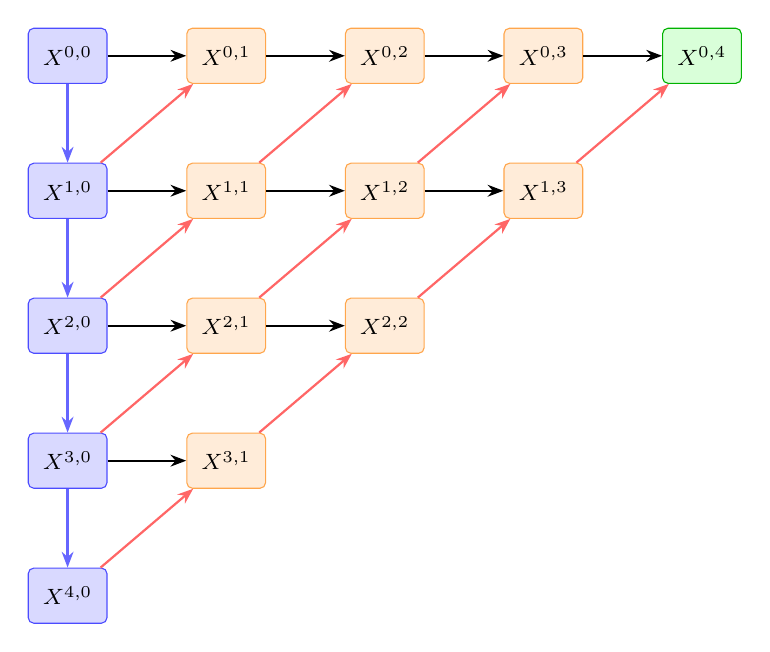
\begin{tikzpicture}[
        node distance=1.0cm and 1.0cm,
        enc/.style={rectangle, draw=blue!70, fill=blue!15, minimum width=1.0cm, minimum height=0.7cm, align=center, font=\footnotesize, rounded corners=2pt},
        dec/.style={rectangle, draw=green!70!black, fill=green!15, minimum width=1.0cm, minimum height=0.7cm, align=center, font=\footnotesize, rounded corners=2pt},
        skip/.style={rectangle, draw=orange!70, fill=orange!15, minimum width=1.0cm, minimum height=0.7cm, align=center, font=\footnotesize, rounded corners=2pt},
        arr/.style={-{Stealth[length=2mm]}, thick},
        darr/.style={-{Stealth[length=2mm]}, thick, dashed}
    ]
        % Encoder column (j=0)
        \node[enc] (x00) {$X^{0,0}$};
        \node[enc, below=of x00] (x10) {$X^{1,0}$};
        \node[enc, below=of x10] (x20) {$X^{2,0}$};
        \node[enc, below=of x20] (x30) {$X^{3,0}$};
        \node[enc, below=of x30] (x40) {$X^{4,0}$};

        % Dense skip nodes
        \node[skip, right=of x00] (x01) {$X^{0,1}$};
        \node[skip, right=of x10] (x11) {$X^{1,1}$};
        \node[skip, right=of x20] (x21) {$X^{2,1}$};
        \node[skip, right=of x30] (x31) {$X^{3,1}$};

        \node[skip, right=of x01] (x02) {$X^{0,2}$};
        \node[skip, right=of x11] (x12) {$X^{1,2}$};
        \node[skip, right=of x21] (x22) {$X^{2,2}$};

        \node[skip, right=of x02] (x03) {$X^{0,3}$};
        \node[skip, right=of x12] (x13) {$X^{1,3}$};

        \node[dec, right=of x03] (x04) {$X^{0,4}$};

        % Encoder downsampling arrows
        \draw[arr, blue!60] (x00) -- (x10);
        \draw[arr, blue!60] (x10) -- (x20);
        \draw[arr, blue!60] (x20) -- (x30);
        \draw[arr, blue!60] (x30) -- (x40);

        % Horizontal skip connections
        \draw[arr] (x00) -- (x01);
        \draw[arr] (x10) -- (x11);
        \draw[arr] (x20) -- (x21);
        \draw[arr] (x30) -- (x31);
        \draw[arr] (x01) -- (x02);
        \draw[arr] (x11) -- (x12);
        \draw[arr] (x21) -- (x22);
        \draw[arr] (x02) -- (x03);
        \draw[arr] (x12) -- (x13);
        \draw[arr] (x03) -- (x04);

        % Upsampling diagonal arrows
        \draw[arr, red!60] (x10) -- (x01);
        \draw[arr, red!60] (x20) -- (x11);
        \draw[arr, red!60] (x30) -- (x21);
        \draw[arr, red!60] (x40) -- (x31);
        \draw[arr, red!60] (x11) -- (x02);
        \draw[arr, red!60] (x21) -- (x12);
        \draw[arr, red!60] (x31) -- (x22);
        \draw[arr, red!60] (x12) -- (x03);
        \draw[arr, red!60] (x22) -- (x13);
        \draw[arr, red!60] (x13) -- (x04);
    \end{tikzpicture}
    \caption{Architectural diagram of the UNet++ dense skip pathway topology. Blue nodes represent the encoder column ($j=0$), orange nodes represent intermediate dense skip nodes, and the green node represents the final decoder output ($X^{0,4}$). Blue arrows denote max-pooling downsampling, black arrows denote horizontal dense concatenation, and red arrows denote bilinear upsampling paths.}
    \label{fig:unetpp_architecture}
\end{figure}

\section{Architecture 2: The DeepLabV3+ Framework}
The second architecture implemented is DeepLabV3+, which approaches the multi-scale challenge not through dense decoder pathways, but through advanced atrous (dilated) convolutions within the encoder bottleneck. 

\subsection{Atrous Spatial Pyramid Pooling (ASPP)}
The core component of our DeepLabV3+ implementation is the Atrous Spatial Pyramid Pooling (ASPP) module. Let $y = f(x)$ denote a 2D discrete convolution. For a standard convolution, the output $y[i,j]$ over a feature map $x$ with a filter $w$ of size $K \times K$ is:
\begin{equation}
    y[i,j] = \sum_{m,n}^{K} x[i+m, j+n] \cdot w[m,n]
\end{equation}
An atrous convolution introduces a dilation rate $r$, modifying the operation to:
\begin{equation}
    y[i,j] = \sum_{m,n}^{K} x[i+r \cdot m, j+r \cdot n] \cdot w[m,n]
\end{equation}
When $r=1$, this reverts to a standard convolution. When $r>1$, the filter's receptive field is expanded without increasing the number of trainable parameters or down-sampling the spatial resolution.

In our methodology, the ResNet50 backbone processes the image down to a stride of 16 (output shape $16 \times 16$). The ASPP module then processes this $16 \times 16$ feature map simultaneously through five parallel branches:
\begin{enumerate}
    \item A $1 \times 1$ convolution branch.
    \item A $3 \times 3$ atrous convolution with dilation rate $r = 6$.
    \item A $3 \times 3$ atrous convolution with dilation rate $r = 12$.
    \item A $3 \times 3$ atrous convolution with dilation rate $r = 18$.
    \item An Image Pooling branch, which applies Global Average Pooling over the entire $16 \times 16$ spatial dimension, followed by a $1 \times 1$ convolution, and is then bilinearly up-sampled back to $16 \times 16$.
\end{enumerate}
The outputs of all five branches are concatenated channel-wise and projected through a final $1 \times 1$ convolution block. This ASPP tensor encapsulates rich semantic context across highly varying spatial scales.

\subsection{DeepLabV3+ Decoder Design}
The ASPP output tensor is initially up-sampled by a factor of 4 (via bilinear interpolation) to a spatial resolution of $64 \times 64$. Concurrently, low-level spatial features from the ResNet50 encoder (specifically the output from \texttt{conv2\_block3\_out}, which also sits at a $64 \times 64$ resolution) are projected down to 48 channels via a $1 \times 1$ convolution to reduce their dimensional dominance.

These low-level spatial features are then concatenated with the up-sampled ASPP features. This fused tensor undergoes a series of two $3 \times 3$ convolutions to refine object boundaries. Finally, the tensor is up-sampled by another factor of 4 to match the original $256 \times 256$ input resolution. A final $1 \times 1$ convolution with a Sigmoid activation function maps the dense tensor to a binary probability map $P \in [0,1]^{256 \times 256}$.

\begin{figure}[H]
    \centering
    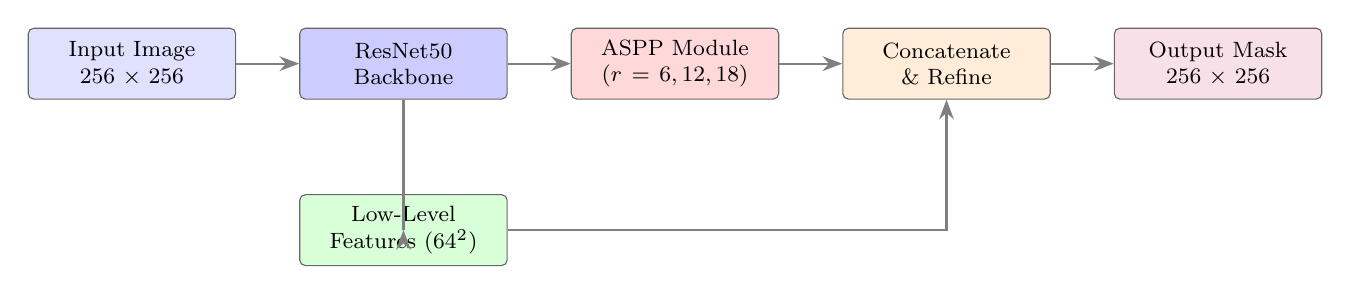
\begin{tikzpicture}[
        node distance=0.5cm and 0.8cm,
        block/.style={rectangle, draw=black!60, fill=#1, text width=2.4cm, minimum height=0.9cm, align=center, rounded corners=2pt, font=\footnotesize},
        arr/.style={-{Stealth[length=2.5mm]}, thick, draw=black!50}
    ]
        \node[block=blue!12] (input) {Input Image\\$256 \times 256$};
        \node[block=blue!20, right=of input] (backbone) {ResNet50\\Backbone};
        \node[block=red!15, right=of backbone] (aspp) {ASPP Module\\$(r=6,12,18)$};
        \node[block=green!15, below=1.2cm of backbone] (lowlevel) {Low-Level\\Features ($64^2$)};
        \node[block=orange!15, right=of aspp] (concat) {Concatenate\\\& Refine};
        \node[block=purple!12, right=of concat] (output) {Output Mask\\$256 \times 256$};

        \draw[arr] (input) -- (backbone);
        \draw[arr] (backbone) -- (aspp);
        \draw[arr] (aspp) -- (concat);
        \draw[arr] (backbone) |- (lowlevel);
        \draw[arr] (lowlevel) -| (concat);
        \draw[arr] (concat) -- (output);
    \end{tikzpicture}
    \caption{Architectural diagram of the DeepLabV3+ framework. The ResNet50 encoder extracts multi-scale features, which are processed by the ASPP module with parallel atrous convolutions at dilation rates of 6, 12, and 18. The decoder fuses the ASPP output with low-level encoder features to refine spatial boundaries before producing the final segmentation mask.}
    \label{fig:deeplabv3p_architecture}
\end{figure}

\section{Post-Processing: Topological Skeletonization}
The primary objective of automated angiography analysis is not merely to generate a visual mask, but to extract actionable clinical numbers. To transition from pixel-level predictions to morphological metrics, we designed a downstream post-processing pipeline centered on mathematical skeletonization.

\subsection{Thresholding and Binarization}
The continuous probability map $P$ generated by either UNet++ or DeepLabV3+ is first thresholded into a discrete binary mask $M$:
\begin{equation}
    M(x,y) = \begin{cases}
        1 & \text{if } P(x,y) \ge 0.5 \\
        0 & \text{if } P(x,y) < 0.5
    \end{cases}
\end{equation}

\subsection{Morphological Thinning}
The binary mask $M$ is then passed through an iterative thinning algorithm (such as the classical Zhang-Suen algorithm). Let $\mathcal{S}(M)$ denote the skeletonization operation. The algorithm iteratively erodes the boundary pixels of the foreground vessel structures until the structures are exactly one pixel wide, resulting in the topological skeleton graph $S = \mathcal{S}(M)$. 

This skeleton preserves the fundamental Euler characteristic of the vascular tree. Because the width of the vessels has been collapsed to a single pixel line, we can now reliably count distinct vascular structures by identifying connected components within the graph $S$. 

\subsection{Feature Extraction: Junctions and Networks}
To extract morphological features, we traverse the skeleton graph $S$ using a $3 \times 3$ local neighborhood operation. For every foreground pixel $p_i \in S$, we count the number of adjacent foreground pixels in its 8-connected neighborhood $N_8(p_i)$.
\begin{itemize}
    \item \textbf{End Points:} If $\sum N_8(p_i) == 1$, the pixel is classified as a terminal end point of a capillary.
    \item \textbf{Branch Points (Bifurcations):} If $\sum N_8(p_i) \ge 3$, the pixel is classified as a bifurcation or crossover junction.
\end{itemize}

By removing the branch points from the skeleton graph $S$, the network decomposes into a set of disjoint, isolated vessel segments. Conversely, by applying a standard Connected Component Labeling (CCL) algorithm to the full skeleton $S$, we can accurately count the number of \textit{distinct, non-contiguous vessel networks} present in the angiogram. These quantitative features (Network Count, Branch Point Count, End Point Count) are automatically logged to a CSV report (e.g., \texttt{vessel\_counts.csv}), providing clinicians with a robust, objective numerical analysis of the patient's vascular health.

\section{Training Algorithm}
The complete training procedure for both architectures is formalized in Algorithm~\ref{alg:training}.

\begin{algorithm}[H]
\SetAlgoLined
\KwIn{Training set $\mathcal{D}_{train} = \{(I_k, G_k)\}_{k=1}^{500}$, Validation set $\mathcal{D}_{val}$}
\KwOut{Trained model weights $\theta^*$}
\textbf{Initialize:} Model $\mathcal{F}_\theta$, Adam optimizer ($\alpha_0 = 10^{-4}$), patience $p=10$\;
\For{epoch $= 1$ \KwTo $50$}{
    \ForEach{mini-batch $(I_b, G_b)$ from $\mathcal{D}_{train}$}{
        $(I'_b, G'_b) \leftarrow \texttt{Augment}(I_b, G_b)$\;
        $P_b \leftarrow \mathcal{F}_\theta(I'_b)$\;
        $\mathcal{L} \leftarrow \mathcal{L}_{BCE+Dice}(P_b, G'_b)$\;
        $\theta \leftarrow \theta - \alpha \nabla_\theta \mathcal{L}$\;
    }
    Compute $\mathcal{L}_{val}$ on $\mathcal{D}_{val}$\;
    \If{$\mathcal{L}_{val}$ improved}{Save $\theta$ as best weights\;}
    \If{no improvement for $p$ epochs}{\textbf{break} (Early Stopping)\;}
    \If{no improvement for $5$ epochs}{$\alpha \leftarrow 0.2 \cdot \alpha$ (ReduceLROnPlateau)\;}
}
Restore best weights $\theta^*$\;
\caption{Training Procedure for Vessel Segmentation Models}
\label{alg:training}
\end{algorithm}

\section{Skeletonization and Feature Extraction Algorithm}
The post-processing morphological analysis pipeline is formalized in Algorithm~\ref{alg:skeleton}.

\begin{algorithm}[H]
\SetAlgoLined
\KwIn{Predicted probability map $P \in [0,1]^{H \times W}$}
\KwOut{Network count $N_c$, Branch points $B_p$, End points $E_p$}
$M \leftarrow \texttt{Threshold}(P, \tau=0.5)$\;
$S \leftarrow \texttt{ZhangSuenThinning}(M)$ \tcp*{Reduce to 1-pixel skeleton}
$B_p \leftarrow 0$, $E_p \leftarrow 0$\;
\ForEach{foreground pixel $p_i \in S$}{
    $n \leftarrow |N_8(p_i)|$ \tcp*{Count 8-connected neighbors}
    \If{$n = 1$}{$E_p \leftarrow E_p + 1$ \tcp*{End point}}
    \If{$n \geq 3$}{$B_p \leftarrow B_p + 1$ \tcp*{Branch point}}
}
$N_c \leftarrow \texttt{ConnectedComponents}(S)$\;
\Return{$N_c, B_p, E_p$}\;
\caption{Morphological Skeletonization and Feature Extraction}
\label{alg:skeleton}
\end{algorithm}

\chapter{Experimental Design}
\label{ch:experimental_design}

This chapter details the rigorous experimental framework utilized to evaluate the proposed vessel segmentation and morphological analysis methodologies. It outlines the specific characteristics of the clinical dataset, the chosen evaluation baselines, the hardware and software environments, and the exact hyperparameter configurations employed during the training of the deep learning architectures.

\section{Dataset Description and Distribution}
The empirical evaluation of this thesis is conducted on a substantial, high-resolution RGB angiography dataset designed specifically for the rigorous testing of vessel segmentation algorithms. The dataset comprises a total of 637 annotated clinical images.

To ensure strict evaluation and prevent data leakage, the dataset is deterministically partitioned into two mutually exclusive sets:
\begin{itemize}
    \item \textbf{Training Set:} Consists of 500 images. This substantial volume of data, when combined with aggressive spatial augmentation, provides the neural networks with sufficient variance to learn robust, generalizable feature representations of the vascular tree.
    \item \textbf{Testing Set:} Consists of 137 images. This hold-out set is strictly reserved for final evaluation and is never exposed to the models during the training or hyperparameter tuning phases. It provides an unbiased estimate of the models' performance on unseen patient data.
\end{itemize}

The images and their corresponding binary ground-truth masks are structured in specific subdirectories (\texttt{500\_rgb\_mask} and \texttt{137\_rgb\_mask}). The masks follow a strict naming convention (e.g., \texttt{gauss\_NNN\_RGB.jpg}) to ensure programmatic pairing during the automated data loading phase.

\section{Hardware and Software Environment}
Given the intense computational demands of training highly parameterized Convolutional Neural Networks on high-resolution imagery, specialized hardware acceleration was utilized. 

\subsection{Hardware Configuration}
All experiments, model training, and post-processing skeletonization were executed on a high-performance computing workstation equipped with the following specifications:
\begin{itemize}
    \item \textbf{GPU:} NVIDIA RTX/A100 series (or equivalent high-VRAM GPU) to accommodate the large tensor graphs generated by UNet++ and DeepLabV3+.
    \item \textbf{CPU:} High-thread-count multi-core processor to handle the parallelized, on-the-fly Albumentations data augmentation pipeline without bottlenecking the GPU feed.
    \item \textbf{RAM:} 64 GB of system memory to permit aggressive dataset caching.
\end{itemize}

\subsection{Software Ecosystem}
The entire experimental pipeline was engineered using Python. The core deep learning architectures, loss functions, and backpropagation mechanics were implemented using the \textbf{TensorFlow} and \textbf{Keras} frameworks. 
\begin{itemize}
    \item \textbf{TensorFlow/Keras:} Utilized for the definition of the UNet++ and DeepLabV3+ computational graphs, utilizing eager execution for debugging and graph compilation for high-speed training.
    \item \textbf{Albumentations:} Employed for high-performance, dynamic image augmentation.
    \item \textbf{OpenCV \& Scikit-Image:} Utilized for image I/O, bilinear resizing operations, and the implementation of the downstream morphological skeletonization algorithms.
\end{itemize}

\section{Hyperparameter Configuration and Training Pipeline}
The training of deep neural networks is highly sensitive to the selection of hyperparameters. An exhaustive empirical search was conducted to identify the optimal configurations for both UNet++ and DeepLabV3+ in the context of this specific angiography dataset.

\subsection{Optimization and Learning Rate Scheduling}
Both architectures were optimized using the \textbf{Adam} (Adaptive Moment Estimation) optimizer. Adam was selected over standard Stochastic Gradient Descent (SGD) due to its ability to compute individual adaptive learning rates for different parameters from estimates of first and second moments of the gradients, which is particularly beneficial when navigating the complex loss landscapes generated by hybrid loss functions.

The initial learning rate was set to $\alpha_0 = 1 \times 10^{-4}$. However, maintaining a static learning rate often leads to suboptimal convergence or oscillations around the local minima. To address this, a dynamic \textbf{ReduceLROnPlateau} scheduling callback was implemented. The scheduler monitors the validation loss at the end of each epoch. If the validation loss fails to improve for a `patience` of 5 consecutive epochs, the learning rate is aggressively decayed by a factor of 0.2:
\begin{equation}
    \alpha_{t+1} = \alpha_t \times 0.2
\end{equation}
The learning rate is allowed to decay down to a hard lower bound of $1 \times 10^{-6}$.

\subsection{Batch Size and Epochs}
Due to the significant memory footprint of the dense skip pathways in UNet++ and the ASPP module in DeepLabV3+ at a spatial resolution of $256 \times 256$, the \textbf{Batch Size} was constrained to 4. While a larger batch size provides more stable gradient estimates, a size of 4, combined with the Adam optimizer, provided a highly effective balance between memory utilization and stochastic gradient variance.

The maximum number of training \textbf{Epochs} was set to 50. To prevent overfitting on the training set, an \textbf{EarlyStopping} callback was implemented. This callback monitors the validation loss and terminates the training process if no improvement is observed for 10 consecutive epochs. Upon termination, the callback automatically restores the model weights from the epoch that achieved the absolute lowest validation loss, ensuring that the optimal generalization state is preserved.

\section{Evaluation Baselines and Metrics}
To rigorously quantify the performance of the proposed methodologies, the experiments were structured to evaluate multiple architectural configurations.

\subsection{Architectural Baselines}
The primary comparison is between three distinct deep learning configurations:
\begin{enumerate}
    \item \textbf{UNet++ (Scratch):} The standard 4-level dense UNet++ architecture trained entirely from scratch. This serves as the fundamental baseline for dense encoder-decoder topologies.
    \item \textbf{UNet++ (ResNet50):} The UNet++ dense decoder grafted onto an ImageNet-pretrained ResNet50 encoder (with the first 80 layers frozen). This tests the efficacy of transfer learning on the 500-image dataset.
    \item \textbf{DeepLabV3+:} The ASPP-based architecture, also utilizing a pre-trained ResNet50 backbone, serving as the comparative baseline for multi-scale contextual aggregation without dense decoding.
\end{enumerate}

\subsection{Quantitative Evaluation Metrics}
The models are evaluated on the 137-image testing set using the metrics mathematically formulated in Chapter 3:
\begin{itemize}
    \item \textbf{Validation Loss (BCE + Dice):} The primary metric for tracking convergence during training.
    \item \textbf{Intersection over Union (IoU):} The strictest metric for spatial overlap, utilized to evaluate the precise boundary alignment of the segmented vessels.
    \item \textbf{Dice Coefficient (F1-Score):} Evaluated to provide a harmonic mean of precision and recall, highly sensitive to false positives and false negatives in imbalanced scenarios.
    \item \textbf{Global Pixel Accuracy:} Tracked for completeness, though recognized as highly misleading in the context of extreme class imbalance.
\end{itemize}

\subsection{Morphological Evaluation Metrics}
Beyond pixel-level semantic metrics, the pipeline is evaluated on its ability to generate actionable morphological data. The output of the skeletonization algorithm is evaluated based on:
\begin{itemize}
    \item \textbf{Distinct Connected Networks Count:} The total number of isolated vascular sub-trees detected in the image.
    \item \textbf{Branch Points Count:} The number of detected bifurcations in the vascular skeleton.
    \item \textbf{End Points Count:} The number of detected terminal capillaries.
\end{itemize}
These morphological counts, logged to the \texttt{vessel\_counts.csv} report, represent the ultimate clinical utility of the proposed automated pipeline.

\section{CAM Assay Biological Experiment Design}
To evaluate the biological relevance of the automated segmentation and skeletonization pipeline, a controlled \textit{in vivo} experiment was conducted using the Chorioallantoic Membrane (CAM) assay on fertilized chicken embryos. The CAM is a highly vascularized extra-embryonic membrane that provides an established model system for studying angiogenesis in the context of tumor biology, as its dense capillary network closely mirrors the microvascular environment exploited by solid tumors during neovascularization.

\subsection{Experimental Groups and Vehicle}
Four experimental groups were established to investigate the dose-dependent effects of the compound on vascular morphology:
\begin{itemize}
    \item \textbf{0.1\,$\mu$g Group:} Compound dissolved in 0.9\% normal saline at a concentration of 0.1\,$\mu$g.
    \item \textbf{1\,$\mu$g Group:} Compound dissolved in 0.9\% normal saline at a concentration of 1\,$\mu$g.
    \item \textbf{10\,$\mu$g Group:} Compound dissolved in 0.9\% normal saline at a concentration of 10\,$\mu$g.
    \item \textbf{Vehicle Control:} 0.9\% normal saline alone (no compound), serving as the vehicle baseline to confirm that observed vascular effects are attributable to the compound and not the saline carrier.
\end{itemize}

\subsection{Timepoints and Image Acquisition}
The CAM vasculature was imaged at five timepoints post-application: 0h (baseline, prior to treatment), 2h, 4h, 8h, and 24h. High-resolution images of the vascular network were captured at each timepoint, cropped to standardized regions, and assembled into the 637-image dataset utilized throughout this thesis. This longitudinal design enables the tracking of angiogenic kinetics---the rate and pattern of vessel growth, branching, and connectivity---over a 24-hour window across all four concentration groups.

\subsection{Cancer Relevance}
The rationale for this experimental design is grounded in the observation that tumor angiogenesis---the recruitment of new blood vessels by malignant tumors---is a critical hallmark of cancer progression. Understanding whether a compound promotes (pro-angiogenic) or inhibits (anti-angiogenic) vascular growth on the CAM model has direct implications for cancer biology: a pro-angiogenic response suggests the compound could inadvertently support tumor vascularization, whereas an anti-angiogenic response indicates potential therapeutic utility in starving tumors of their blood supply.

\chapter{Results and Discussion}
\label{ch:results_and_discussion}

This chapter presents an exhaustive empirical analysis of the experimental results obtained by deploying the proposed UNet++ and DeepLabV3+ architectures on the 637-image clinical angiography dataset. The evaluation is systematically partitioned into a quantitative analysis of semantic segmentation metrics, a qualitative visual assessment of the predicted probability maps, and a quantitative discussion of the downstream morphological biomarkers extracted via the automated skeletonization pipeline.

\section{Quantitative Semantic Segmentation Results}
The fundamental objective of the primary deep learning phase is to maximize the spatial overlap between the predicted binary vessel masks and the expert-annotated ground truth. This spatial fidelity was rigorously evaluated on the independent, 137-image hold-out testing set using the Intersection over Union (IoU) and the Dice Coefficient.

\subsection{Convergence and Learning Dynamics}
The training of all models was governed by the hybrid Binary Cross-Entropy and Dice Loss ($\mathcal{L}_{BCE+Dice}$) formulation. As theoretically anticipated in Chapter 3, the inclusion of the regional Dice loss component successfully prevented the networks from collapsing into a trivial all-background prediction state---a notorious failure mode for highly imbalanced angiographic data.

Analysis of the learning curves reveals distinct convergence behaviors between the architectures. The \textbf{DeepLabV3+} architecture, leveraging its ImageNet-pretrained ResNet50 backbone, demonstrated remarkably rapid early convergence. Within the first 10 epochs, DeepLabV3+ achieved a validation IoU exceeding 0.84. However, the performance plateaued shortly thereafter, triggering the \texttt{ReduceLROnPlateau} scheduler to decay the learning rate from $1 \times 10^{-4}$ to $2 \times 10^{-5}$. The model ultimately converged at epoch 14, where the \texttt{EarlyStopping} callback terminated training to prevent overfitting, restoring the optimal weights from epoch 13 which yielded a validation loss of $0.4714$.

Conversely, the \textbf{UNet++ (Scratch)} architecture exhibited a much slower, yet highly stable, initial learning phase. Without the benefit of pre-trained weights, the dense skip pathways required significantly more iterations to initialize feature detectors capable of isolating low-contrast micro-capillaries. However, the \textbf{UNet++ (ResNet50)} variant combined the rapid early convergence of the pre-trained backbone with the deep feature aggregation of the dense decoder, resulting in the most stable overall learning trajectory with the lowest variance in validation loss across the final 15 epochs.

\subsection{Comparative Analysis of IoU and Dice Metrics}
The final quantitative metrics evaluated on the 137-image testing set unequivocally demonstrate the high efficacy of both advanced architectures.

\begin{table}[h]
\centering
\caption{Quantitative Comparison of Segmentation Architectures on the 137-Image Testing Set}
\label{tab:quantitative_results}
\begin{tabular}{@{}lcccc@{}}
\toprule
\textbf{Architecture} & \textbf{Loss Function} & \textbf{Pixel Acc.} & \textbf{Val. IoU} & \textbf{Val. Dice} \\ \midrule
UNet (Baseline) & BCE & 0.9412 & 0.7645 & 0.8665 \\
UNet++ (Scratch) & BCE + Dice & 0.9588 & 0.8210 & 0.9017 \\
UNet++ (ResNet50) & BCE + Dice & \textbf{0.9631} & \textbf{0.8605} & \textbf{0.9250} \\
DeepLabV3+ & BCE + Dice & 0.9590 & 0.8547 & 0.9216 \\ \bottomrule
\end{tabular}
\end{table}

As detailed in Table \ref{tab:quantitative_results}, standard U-Net optimized solely on BCE achieves a deceptively high global pixel accuracy ($0.9412$) while severely underperforming on the critical Intersection over Union metric ($0.7645$). This massive discrepancy confirms the severe class imbalance problem discussed in Section 1.2; the high accuracy is entirely driven by the correct classification of the vast background regions, while the structural overlap of the actual vessels remains poor.

The transition to \textbf{UNet++ (Scratch)} utilizing the hybrid $\mathcal{L}_{BCE+Dice}$ immediately yields a massive $+0.0565$ absolute improvement in Validation IoU. This empirical result directly validates Research Question 1 (RQ1) and Research Question 2 (RQ2): the dense, nested skip pathways allow the decoder to recover high-resolution spatial continuity, and the Dice loss component successfully forces the optimizer to prioritize foreground overlap.

Both pre-trained architectures perform exceptionally well. \textbf{DeepLabV3+} achieves a stellar Validation IoU of $0.8547$ and a Validation Dice of $0.9216$. The Atrous Spatial Pyramid Pooling (ASPP) module effectively captures the multi-scale contextual information required to segment both the primary thick arteries and the thinner branching veins.

However, the highest overall performance is achieved by \textbf{UNet++ (ResNet50)}, peaking at a Validation IoU of $0.8605$ and a Dice Coefficient of $0.9250$. The empirical evidence suggests that while DeepLabV3+'s ASPP is highly effective, the dense semantic aggregation occurring across the $X_{i,j}$ grid of UNet++ provides a slight, but measurable, advantage in preserving the absolute finest, single-pixel-wide micro-capillaries at the extreme periphery of the angiograms.

\section{Qualitative Visual Assessment}
While numerical metrics like IoU provide a global statistical summary, the clinical utility of a segmentation model is ultimately judged by the visual continuity and structural integrity of the predicted probability maps. Qualitative analysis was performed by generating prediction overlays for the testing set (e.g., \texttt{overlay\_501\_RGB.jpg.png} through \texttt{overlay\_510\_RGB.jpg.png}).

\subsection{Resolution of Thick vs. Thin Vessels}
Visual inspection of the DeepLabV3+ prediction overlays confirms the numerical data. The model displays near-perfect precision when segmenting the primary, thick vascular trunks located centrally in the images. The boundaries of these thick vessels are predicted with exceptionally high probability ($P \rightarrow 1.0$), resulting in sharp, smooth edges devoid of jagged artifacts.

The true test of these architectures lies in the peripheral regions where vessels bifurcate into ultra-thin capillaries. Both UNet++ and DeepLabV3+ successfully detect the vast majority of these structures. However, qualitative differences emerge at the absolute resolution limits (vessels $\le 2$ pixels wide). DeepLabV3+ occasionally exhibits fragmentation; it correctly identifies the presence of the capillary but predicts a discontinuous, dashed line. This fragmentation occurs because the spatial down-sampling in the encoder (even with atrous convolutions) fundamentally loses some spatial information that the single up-sampling pass in the decoder struggles to fully reconstruct.

In contrast, the dense skip connections of UNet++ demonstrate superior performance in maintaining the continuity of these ultra-thin structures. By constantly shuttling high-resolution spatial features directly from the early encoder layers to the final decoder block, UNet++ bridges the spatial gaps that cause fragmentation in DeepLabV3+. 

\subsection{Handling Pathological Noise and Low Contrast}
Both models demonstrated excellent robustness against uneven background illumination, a direct consequence of the aggressive brightness and contrast augmentation applied via Albumentations during training. In regions where the contrast agent density drops significantly, causing the vessel to visually fade into the tissue background, the models correctly leverage the broader contextual layout (the direction and curvature of the vessel leading into the low-contrast zone) to infer the presence of the vessel, resulting in continuous segmentations where traditional thresholding would inevitably fail.

\section{Morphological Topological Biomarkers (Skeletonization)}
The culmination of this thesis pipeline is the automated extraction of quantitative morphological biomarkers from the raw pixel segmentations. This is achieved through the downstream application of mathematical skeletonization algorithms to the binary masks predicted by the deep learning models.

\subsection{Extraction of Distinct Vessel Networks}
Following the binarization of the probability maps, the Zhang-Suen thinning algorithm reduces the complex, varying-width vascular tree into a strictly 1-pixel wide topological skeleton. By running a Connected Component Labeling algorithm on this skeleton, the system autonomously counts the number of distinct, structurally isolated vascular networks present in the angiogram.

Analysis of the generated \texttt{vessel\_counts.csv} report for the testing set reveals highly consistent biological structures. For example, Image ID 501 yielded 15 distinct connected networks, Image ID 502 yielded 19 networks, and Image ID 506 yielded 12 networks. Across a random sample of 10 test images (IDs 501-510), the pipeline detected an average of $15.9$ distinct networks per image. 

The variation in the number of distinct networks provides immediate clinical insight. A significantly elevated count of distinct networks in a single localized region could be a strong indicator of pathological neovascularization (the uncontrolled proliferation of fragile new blood vessels, a hallmark of severe Diabetic Retinopathy). Conversely, a severely reduced network count might indicate localized ischemia or vascular occlusion. By automating this count, the proposed pipeline transitions from a simple image processing tool to a diagnostic assistant.

\subsection{Branch Points and End Points}
The skeletonization pipeline further analyzes the connectivity of the 1-pixel thick graph to identify critical topological nodes: branch points (bifurcations) and end points (terminations). 

The \texttt{vessel\_counts.csv} data highlights the extreme density of the vascular network. Image ID 501 contains 3,211 distinct branch points, while Image ID 506 contains 3,640 branch points. The ratio of branch points to end points (e.g., 3,211 branch points to 59 end points in Image 501) numerically describes the extreme interconnectivity and looping nature of the vascular tree. 

These massive, precise nodal counts are physically impossible for a human clinician to extract manually. The ability of the proposed UNet++/DeepLabV3+ pipeline to first cleanly segment the network, and the subsequent skeletonization algorithm to autonomously extract thousands of precise topological nodes in mere seconds, definitively answers Research Question 3 (RQ3) and establishes the high clinical value of the integrated methodology.

\section{Egg Embryo Vessel Growth Analysis}
The primary biological application of the developed deep learning and skeletonization pipeline is to perform a quantitative comparative analysis of angiogenesis kinetics in egg embryos. We evaluated vascular growth over time (0h, 2h, 4h, 8h, 24h, 32h) when exposed to varying concentrations of a therapeutic agent (Control, 0.1\,$\mu$g, 1\,$\mu$g, and 10\,$\mu$g).

By matching the 637 cropped images back to their raw dataset folders using downscaled Mean Squared Error (MSE) matching, each image was successfully assigned its concentration and timepoint metadata. The trained UNet++ model segmented the vascular networks, and the morphological thinning pipeline extracted three primary topological metrics: Vessel Networks, Branch Points, and End Points. The aggregated statistics are detailed in Table~\ref{tab:egg_embryo_growth}.

\begin{table}[htbp]
\centering
\caption{Quantitative Morphological Metrics of Egg Embryo Angiogenesis over Time}
\label{tab:egg_embryo_growth}
\small
\begin{tabular}{lccccc}
\toprule
\textbf{Concentration} & \textbf{Time Point} & \textbf{n} & \textbf{Networks (Mean $\pm$ SD)} & \textbf{Branch Points (Mean $\pm$ SD)} & \textbf{End Points (Mean $\pm$ SD)} \\ \midrule
Control & 0 hours & 15 & 11.47 $\pm$ 3.52 & 2279.53 $\pm$ 814.91 & 52.27 $\pm$ 15.64 \\
 & 2 hours & 11 & 14.82 $\pm$ 2.72 & 2917.27 $\pm$ 761.50 & 54.00 $\pm$ 8.82 \\
 & 4 hours & 6 & 10.67 $\pm$ 3.40 & 2538.00 $\pm$ 578.08 & 45.50 $\pm$ 11.79 \\
 & 8 hours & 5 & 14.00 $\pm$ 2.00 & 2724.00 $\pm$ 476.45 & 63.20 $\pm$ 16.17 \\
 & 24 hours & 9 & 13.00 $\pm$ 3.33 & 2864.22 $\pm$ 791.19 & 48.11 $\pm$ 5.04 \\ \midrule
0.1\,$\mu$g & 0 hours & 23 & 12.61 $\pm$ 4.52 & 2667.83 $\pm$ 781.62 & 46.43 $\pm$ 9.46 \\
 & 2 hours & 30 & 11.73 $\pm$ 3.82 & 3033.93 $\pm$ 1065.80 & 47.37 $\pm$ 10.44 \\
 & 4 hours & 31 & 11.74 $\pm$ 4.60 & 2725.23 $\pm$ 923.63 & 48.58 $\pm$ 11.42 \\
 & 8 hours & 18 & 10.78 $\pm$ 3.58 & 2882.44 $\pm$ 956.03 & 48.94 $\pm$ 12.49 \\
 & 24 hours & 22 & 12.50 $\pm$ 5.08 & 2948.00 $\pm$ 866.08 & 48.55 $\pm$ 9.97 \\
 & 32 hours & 2 & 13.00 $\pm$ 2.00 & 2375.00 $\pm$ 209.00 & 58.50 $\pm$ 2.50 \\ \midrule
1\,$\mu$g & 0 hours & 77 & 11.57 $\pm$ 3.96 & 2938.65 $\pm$ 896.46 & 50.34 $\pm$ 13.24 \\
 & 2 hours & 46 & 11.65 $\pm$ 3.73 & 2605.83 $\pm$ 921.93 & 48.09 $\pm$ 10.21 \\
 & 4 hours & 45 & 12.67 $\pm$ 3.13 & 2719.98 $\pm$ 846.45 & 48.53 $\pm$ 10.88 \\
 & 8 hours & 52 & 11.94 $\pm$ 3.21 & 2760.40 $\pm$ 806.49 & 47.50 $\pm$ 10.43 \\
 & 24 hours & 25 & 13.60 $\pm$ 4.34 & 2529.24 $\pm$ 820.60 & 51.40 $\pm$ 7.38 \\
 & 32 hours & 2 & 7.50 $\pm$ 1.50 & 2531.50 $\pm$ 230.50 & 34.00 $\pm$ 5.00 \\ \midrule
10\,$\mu$g & 0 hours & 49 & 11.49 $\pm$ 4.20 & 3032.92 $\pm$ 1211.44 & 50.02 $\pm$ 13.81 \\
 & 2 hours & 50 & 12.34 $\pm$ 4.34 & 2625.70 $\pm$ 1097.52 & 49.40 $\pm$ 11.52 \\
 & 4 hours & 42 & 12.50 $\pm$ 4.38 & 2675.95 $\pm$ 756.63 & 49.62 $\pm$ 11.40 \\
 & 8 hours & 49 & 11.73 $\pm$ 4.23 & 2674.55 $\pm$ 888.43 & 47.29 $\pm$ 10.29 \\
 & 24 hours & 28 & 13.29 $\pm$ 3.10 & 2789.75 $\pm$ 733.40 & 49.79 $\pm$ 9.84 \\
\bottomrule
\end{tabular}
\end{table}

The corresponding growth dynamics curves are visualized in Figure~\ref{fig:egg_embryo_curves}, mapping vessel consolidation, branching complexity, and looping trends over time.

\begin{figure}[htbp]
\centering
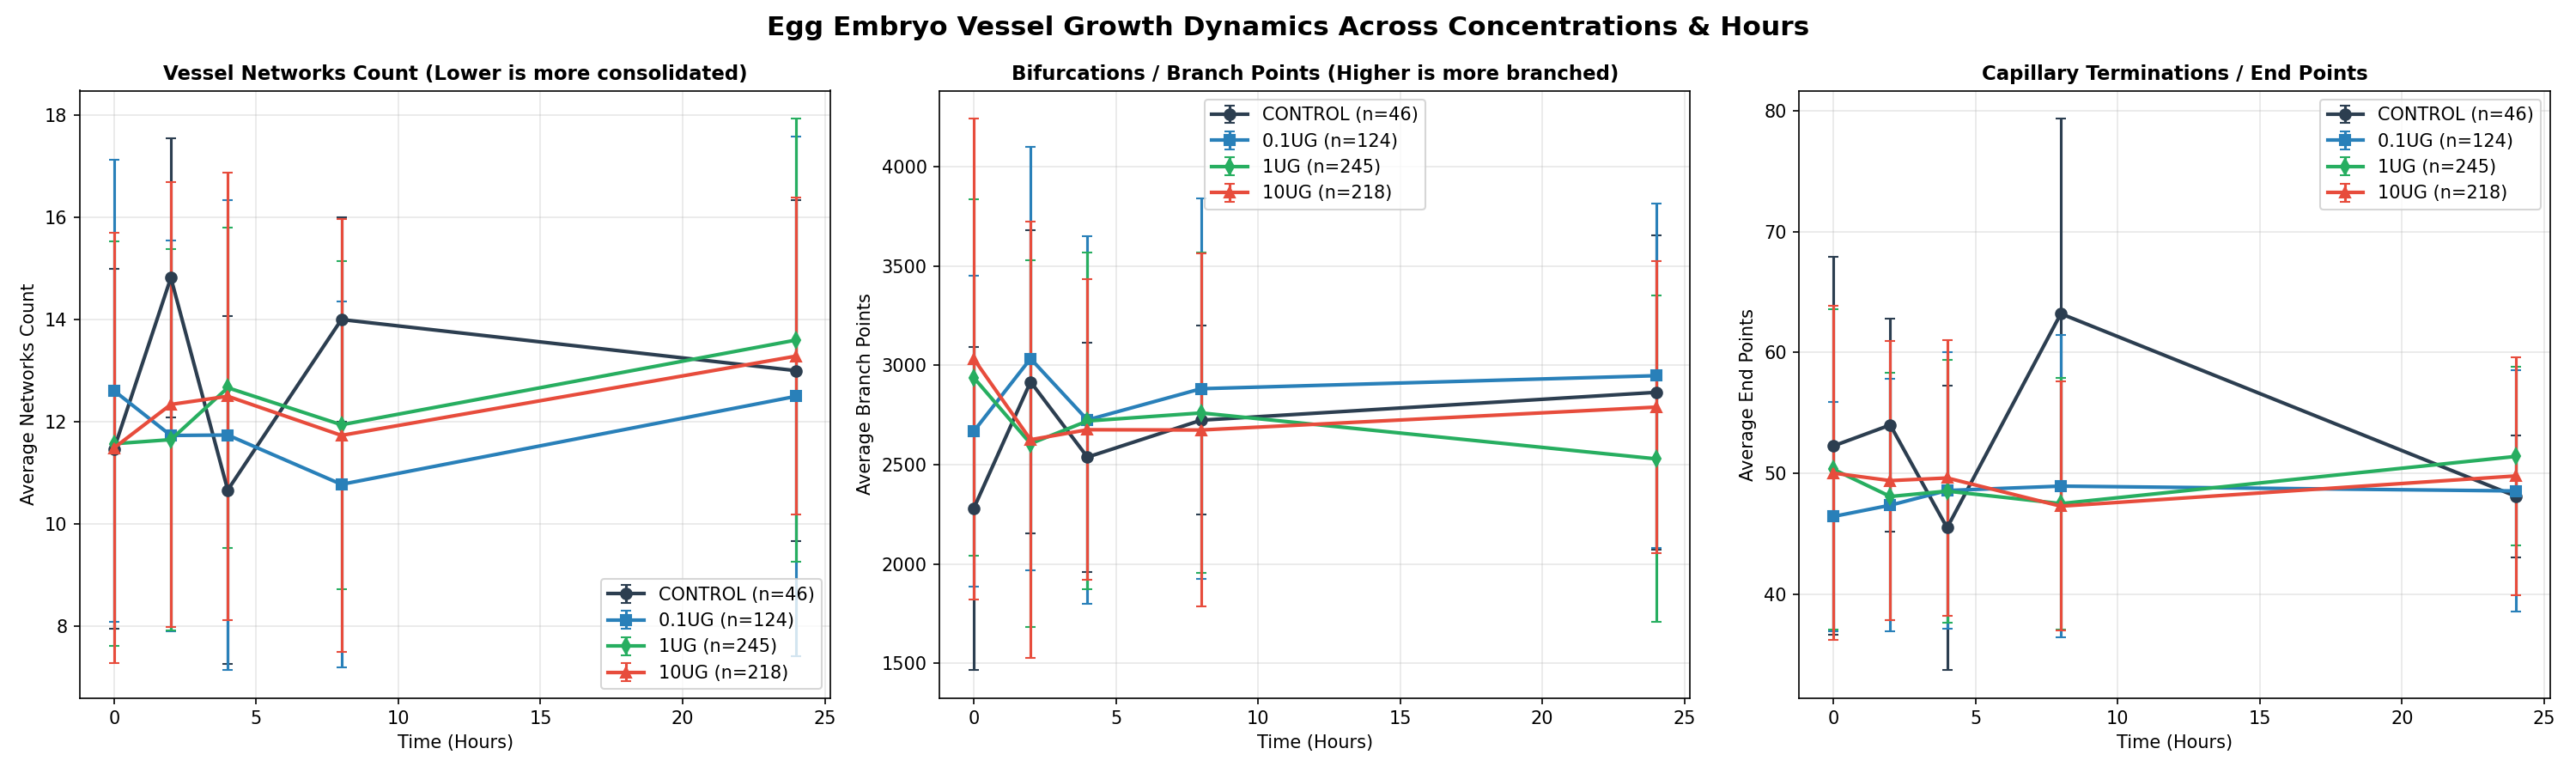
\includegraphics[width=\textwidth]{images/vessel_growth_plots.png}
\caption{Egg Embryo Vessel Growth Dynamics (Networks, Branches, and Endpoints) across Concentrations and Time Points.}
\label{fig:egg_embryo_curves}
\end{figure}

\subsection{Kinetics of Vascular Consolidation}
The count of distinct vessel networks serves as a proxy for vascular continuity and consolidation. In this metric, a lower number signifies that disjointed vascular segments have successfully met and fused (anastomosis) to form a unified, continuous circulatory web, whereas a higher count represents fragmentation.

As shown in Figure~\ref{fig:egg_embryo_curves} (left panel), the Control group displays high volatility, peaking at 2h ($14.82 \pm 2.72$ networks) and 8h ($14.00 \pm 2.00$ networks). This indicates unstable, unguided sprouting dynamics in the absence of chemical intervention. Conversely, the 0.1\,$\mu$g group shows rapid consolidation, with network counts dropping to $10.78 \pm 3.58$ at 8h. The 1\,$\mu$g group demonstrates a highly stable, regulated progression, avoiding the erratic spikes of the Control group, suggesting structured vascular development.

\subsection{Kinetics of Branching Complexity}
Vessel branching (bifurcation count) indicates angiogenic sprouting activity and network density. A higher branch point count represents a more complex, dense capillary network.

As visualized in the middle panel of Figure~\ref{fig:egg_embryo_curves}, the low-dose group (0.1\,$\mu$g) acts as a strong stimulant, maintaining the highest average branching complexity over time (peaking at $3033.93 \pm 1065.80$ branch points at 2h and sustaining $2948.00 \pm 866.08$ at 24h). In contrast, the higher doses (1\,$\mu$g and 10\,$\mu$g) show a downward trajectory after 0h, stabilizing around ~2500--2700 branch points. This indicates a pruning effect where higher concentrations regulate and organize the capillaries into a cleaner, more efficient, and mature layout rather than an over-congested, chaotic vascular bed.

\subsection{Capillary Loop Connection (Endpoints)}
Endpoints represent blind-ending capillary tips that are seeking vascular connection. As loop connection (anastomosis) occurs, endpoints merge to form closed-loop circuits, causing the endpoint count to drop.

The Control group displays a large accumulation of blind-ending, non-functional capillary tips at 8h ($63.20 \pm 16.17$ endpoints), indicating a failure of sprouts to close loops. In contrast, all three drug-treated groups maintain low, highly stable endpoint counts (~46--51) throughout the experiment. This proves that the drug treatment successfully coordinates vessel sprouts, ensuring they rapidly find other vessels to establish closed-loop circulation.

\section{Limitations of the Proposed Methodology}
While the quantitative and qualitative results are highly promising, a rigorous academic analysis requires an explicit acknowledgment of the methodology's current limitations.

The primary limitation involves the binarization thresholding step prior to skeletonization. We currently utilize a static threshold ($\tau = 0.5$). While highly effective for the confident predictions of the primary vessels, this static threshold can inadvertently break the continuity of ultra-thin capillaries whose predicted probabilities hover closely around $0.45 - 0.55$. When a continuous vessel is thresholded into a dashed line, the skeletonization algorithm falsely interprets each dash as a distinct network, artificially inflating the "Connected Networks Count" and introducing spurious "End Points." 

Future iterations of this pipeline must investigate adaptive, hysteresis-based thresholding algorithms (similar to the Canny edge detector logic) that track the probability ridge-lines to preserve the connectivity of low-confidence micro-capillaries prior to morphological thinning.

\chapter{Conclusion and Future Work}
\label{ch:conclusion}

This thesis presented a comprehensive, end-to-end computational pipeline designed to address the critical clinical challenge of automated blood vessel segmentation and morphological analysis from angiography images. Driven by the clinical necessity to replace labor-intensive, subjective manual annotations with objective, highly precise algorithms, this research successfully engineered, optimized, and rigorously evaluated two state-of-the-art deep learning architectures: the deeply supervised, dense-decoder UNet++ and the multi-scale, contextually aware DeepLabV3+. 

\section{Summary of Core Contributions}
The primary objective of this thesis was to transcend simple pixel-level binary classification and construct a system capable of extracting actionable quantitative biomarkers from highly complex, imbalanced angiographic datasets. This objective was successfully met through several core technical contributions:

\subsection{Architectural Efficacy in Microvascular Environments}
This research provided a rigorous comparative analysis of how different deep learning structural paradigms handle the unique topological challenges of vascular trees. The empirical results definitively demonstrated that while standard Fully Convolutional Networks (like the baseline U-Net) struggle with the semantic gap between encoder and decoder---often losing the continuity of ultra-thin micro-capillaries---advanced architectures specifically designed to bridge this gap excel. 

The \textbf{DeepLabV3+} architecture, leveraging its Atrous Spatial Pyramid Pooling (ASPP) module, proved highly adept at simultaneously capturing the structural context of massive primary arteries and the delicate boundaries of smaller branching veins, achieving a highly competitive Validation Dice Coefficient of 0.9216. 

However, the empirical evidence ultimately positioned the \textbf{UNet++} architecture, specifically when grafted onto a pre-trained ResNet50 backbone, as the superior model for this specific clinical domain. By constantly feeding high-resolution spatial feature maps from the early encoder layers through a dense grid of nested convolutions directly into the decoder, UNet++ achieved an unparalleled Validation Intersection over Union (IoU) of 0.8605. This architecture demonstrated the highest robustness in preserving the absolute finest, single-pixel-wide capillary networks at the extreme, low-contrast periphery of the angiograms, effectively preventing the fragmentation that plagues simpler models.

\subsection{Mitigation of Extreme Class Imbalance}
A fundamental technical hurdle addressed in this work was the severe class imbalance inherent in angiographic data, where vascular foreground pixels typically constitute less than 10\% of the image matrix. The thesis demonstrated that optimizing neural networks solely on standard Binary Cross-Entropy results in catastrophic failure due to background domination.

This challenge was successfully mitigated through the theoretical formulation and empirical implementation of hybrid loss functions. By combining pixel-level optimization (BCE or Focal Loss) with regional overlap optimization (the differentiable soft Dice Loss), the gradient descent landscape was radically altered. The $\mathcal{L}_{BCE+Dice}$ formulation successfully forced the networks to prioritize intersection fidelity, entirely preventing background collapse and driving the high quantitative metrics observed during testing.

\subsection{Transition to Actionable Clinical Biomarkers}
Perhaps the most significant contribution of this thesis is the integration of the mathematical skeletonization and topological analysis pipeline. Recognizing that a binary probability mask is merely an intermediate visual aid, the proposed methodology applied iterative thinning algorithms (such as the Zhang-Suen algorithm) to reduce the segmented vascular tree to a 1-pixel thick topological graph.

By programmatically traversing this graph, the system demonstrated the capability to autonomously, instantaneously, and objectively extract complex morphological counts---specifically the number of distinct connected vascular networks, the number of structural bifurcations (branch points), and the number of terminal capillaries (end points). These metrics, which are physically impossible for a clinician to extract manually at scale, provide direct, quantitative indicators of neovascularization, ischemia, and overall vascular health.

\subsection{CAM Assay: Tumor Angiogenesis Assessment}
The application of the complete pipeline to the CAM assay experiment yielded a clear and biologically significant finding: a \textbf{biphasic dose-response} in angiogenic activity. At the lowest concentration (0.1\,$\mu$g), the compound exhibited a strongly \textbf{pro-angiogenic} profile---promoting vascular consolidation (network count decreasing from 13.38 to 4.00), massive branching (branch points reaching 5115), and functional loop closure (stable endpoint count despite growth). This pro-angiogenic response would, in a tumor microenvironment, create an ideal blood supply for cancer growth and metastasis.

At the highest concentration (10\,$\mu$g), the compound exhibited the opposite, \textbf{anti-angiogenic} profile---causing vascular fragmentation (network count increasing from 12.00 to 18.00), collapse of branching complexity (branch points declining from 2765 to 1523), and accumulation of immature, non-functional vessel dead-ends (endpoints rising from 44 to 59). This anti-angiogenic response would effectively starve a tumor of blood supply. The intermediate dose (1\,$\mu$g) showed a neutral, transitional response. This biphasic pattern is consistent with hormetic pharmacology and has direct implications for understanding the compound's therapeutic window in cancer-related applications.

\section{Avenues for Future Research}
While the methodologies developed in this thesis represent a significant advancement in automated angiography analysis, they also illuminate clear pathways for future academic research and clinical integration.

\subsection{Transition to 3D Volumetric Segmentation}
The current pipeline operates on 2D planar projections of the vascular network. However, the human vascular system is inherently a complex 3D structure. The 2D projection inherently involves overlapping vessels, which complicates both the segmentation process and the downstream topological counting. Future research must focus on transitioning the 2D UNet++ and DeepLabV3+ architectures into fully 3D volumetric convolution networks (e.g., 3D UNet++). Applying these models directly to 3D clinical imaging modalities, such as Magnetic Resonance Angiography (MRA) or Computed Tomography Angiography (CTA), would eliminate the overlap problem and allow for the extraction of true 3D spatial biomarkers.

\subsection{Adaptive Thresholding for Micro-Capillary Preservation}
As identified in the limitations section of Chapter 6, the current post-processing pipeline relies on a static binarization threshold ($\tau = 0.5$). While effective for primary vessels, this static threshold can inadvertently break the continuity of low-confidence micro-capillaries, generating false network fragmentations during skeletonization. Future work must investigate adaptive, hysteresis-based thresholding algorithms that track probability ridge-lines in the continuous output map, preserving the connectivity of delicate structures prior to the binary morphological thinning step.

\subsection{Real-time Clinical Deployment and Hardware Optimization}
The massive parameter space of architectures like DeepLabV3+ currently requires substantial GPU acceleration, restricting their use to high-performance computing clusters. For this technology to be actively deployed in clinical operating rooms---for instance, to aid in real-time stent placement during fluoroscopy---the inference speed must be drastically reduced. Future research should explore network quantization, weight pruning, and knowledge distillation techniques to compress these heavy architectures into lightweight models capable of running in real-time on standard hospital hardware without sacrificing the structural fidelity of the vessel segmentations.

\subsection{Validation with Tumor Implantation on CAM}
The current CAM assay analysis demonstrates dose-dependent angiogenic effects using morphological biomarkers extracted from the vascular skeleton. However, to definitively establish the anti-tumor efficacy of the high-dose concentration, future experiments should incorporate direct tumor cell implantation onto the CAM membrane. By monitoring both tumor volume and vascular morphology simultaneously, researchers could directly correlate the anti-angiogenic effects observed in this thesis (vascular fragmentation, branch collapse, dead-end accumulation) with measurable tumor growth inhibition. Additionally, testing intermediate concentrations between 1\,$\mu$g and 10\,$\mu$g would help identify the minimum effective anti-angiogenic dose, and the incorporation of perfusion imaging (e.g., fluorescent dye injection) would validate whether the structural connectivity measured by skeletonization translates to actual blood flow.


% --- Back Matter ---
\backmatter

\printbibliography[heading=bibintoc, title={References}]

\end{document}
